\documentclass[12pt]{article}
\usepackage[utf8]{inputenc}

\title{Diffy Q The Laplace Transform}
\author{Connor Scholten}
\date{January 2017}

\usepackage{natbib}
\usepackage{graphicx}
\usepackage{amsmath}
\usepackage{amssymb}
\usepackage{mdsymbol}
\usepackage{mathrsfs}
\usepackage{indentfirst}
\newcommand{\lp}{\mathscr{L}}
\newcommand{\lrsa}{\longrightsquigarrow}
\newcommand{\hugey}{\mathscr{Y}}

\setcounter{tocdepth}{2}  % levels under \subsection are not listed in the TOC

\begin{document}

\maketitle

\pagebreak

\tableofcontents

\pagebreak

\section{Introduction}

In terms of general solution techniques out there for solving Ordinary Differential Equations, like Integrating Factors, Undetermined Coefficients, Reduction of Order, Variation of Parameters, or Series Solutions, each has their moments with abilities to answer certain kinds of equations and the amount of range they have. This will be only about one method, the Laplace Transform, and this method by far reaches further than any other method previously studied. This is usually the favorite method for those using practical applications of Differential Equations. It is a full study that goes beyond what is seen in and introduction of Differential Equations. We will stay in the undergraduate level here, for the material needed in an Intro Differential Equations class, this will cover most lecture topics that get taught in this subject.

\subsection{The Method}

The Laplace transform method will work as follows: \\

1) Starting with the Differential Equation, Transform both sides of the equation with the Laplace Transform. Transforming our Differential Equation into an algebraic equation. \\

2) Solve the algebraic equation and write it into a certain form. \\

3) Take the Inverse Laplace Transform to get back to our needed function to be the answer. \\

We will initially have to study the equivalent of several lectures on the Laplace Transform in sufficient detail of its properties before we can execute this solving method on even the most basic of Differential Equations. We will collect the big properties and put them in a table. Once we have enough properties to see our first Differential Equation solve we will solve our first one, then after that we will see the Laplace method's real abilities. \\

\section{Laplace Transform Definition}

\subsection{Transform vs. Operator}

The first part of the definition we should discuss is, "what is a Transform?" In Mathematics there is this sounding similarity between an operator and a Transform. In essence these two serve the same purpose, changing one or more mathematical objects into something else, learning its properties, then using them to model or solve problems. The subtle difference we need will come when thinking more specifically, narrowing the mathematical objects to being only functions for this context. Consider an operator on a function, $f(t)$, will change the function from $f$ to some other $g$ but the variable will still be the same, $g(t)$. An example of this would be the derivative operator. A Transform is taking $f(t)$ but not only can we change the function but we will change the variable as well, here usually from $t$ to $s$ lets say. That would mean $f(t)$ Transformed to $G(s)$, a simple example of a Transform would be an integral with a new variable as one of the limits of integration, after integrating the old variable will get replaced with the new variable once the limits are substituted. Without further ado, the Laplace part of the Transform will be an integral but specifically the following kind. We denote taking the Transform of a function $f(t)$ into a $F(s)$ as $\lp [f(t)]$, it will be defined as

\begin{equation*}
    \lp[f(t)] = \int_0^{\infty} f(t) e^{-st} dt.
\end{equation*}

It is a very common to denote the Laplace Transform of a function as that function's capital letter, since usually when we integrate a function $f(t)$, we call it $F(t)$, seeing how Laplace is an integral, that will make notation more intuitive. The next part is since it is a Transform we should note after $F$ what the new variable should be, we changed $t$ to $s$ in this Transform which is why Laplace of $f(t)$ is denoted as $F(s)$.

\subsection{Motivating the Definition}

In the study of Laplace Transforms there is a looming mysteriousness of how the Laplace Transform was motivated to be defined this way. There is usually a disconnect between what the Differential Equations student wants as an answer and where did it come from historically. Historically the study came from the study of Moment Generating Functions from probability theory which is only a couple changes away from the Laplace integral. Though the subtle yet better to question ask is what is the most basic motivator for defining the Laplace Transform like this that a typical  Calculus student can handle? The answer boils down to Power Series. \\

Consider a Power Series with unknown coefficients of the form, 

\begin{equation*}
    \sum_0^{\infty} a_nx^n = A(x).
\end{equation*}

The $a_n$, being the coefficients of each term is really just a function that takes values of whole numbers $n$ and designates each $n$ to a real number, so we will slightly change the notation from the usual $a_n$ to $a(n)$ to get us to a subtly different but easier mindset,

\begin{equation*}
    \sum_0^{\infty} a(n)x^n = A(x).
\end{equation*}

So we can think of Power Series like a Transform from $a(n)$ to $A(x)$, which we can also denote this Transform as a maybe more intuitively looking $a(n) \lrsa A(x)$. Consider some examples, like if $a(n)$ is one that is all values of $n=1,2,3, ...$ all are associated with $a(n)=1$, the Power Series of that is $A(x)=1+x+x^2+x^3+...$ this becomes a Geometric Series, which we show a reminder of how it works in our Periodic Functions section much further down. There we will conclude we can rewrite that infinite polynomial as $A(x)=\frac{1}{1-x}$, thus we abbreviate explaining this Transformation concept down to the symbolic $1 \lrsa \frac{1}{1-x}$. However we will also show on the condition that this is only true when $|x|<1$, otherwise we would have an issue with a diverging limit problem. \\

Another example of a Transform like this is if $a(n)=\frac{1}{n!}$, thus it inputs as $\sum_{n=0}^{\infty}\frac{1}{n!}x^n = 1+x+\frac{1}{2!}x^2+\frac{1}{3!}x^3+\ldots$, this is most notably the coefficients for the Taylor series of $e^x$, so that Transform is $\frac{1}{n!} \lrsa e^x$. Notice here the left was a function of integers $n$, and the right is a function of $x$ making it a Transform. Now this Transform works in the Discrete case but we want to know about continuous functions like with real world applications starting with the continuous variable time. That is we want to change our variable definition from being discrete $n=1,2,3,...$ to continuous $0 \leq t \leq \infty$. \\

The continuous analog of the Power Series Transform is not that much of a stretch of being

\begin{equation*}
    \int_0^{\infty} a(t)x^t dt = A(x).
\end{equation*}

We could leave it in this form but it is a painful to integrate functions like this, a base $e$ function has really simple rules for integrating and differentiating so we change the base $x^t=\left(e^{ln(x)}\right)^t$. We should also note that, after all we want to calculate that integral above, when $x \geq 1$ this integral is really unlikely to converge, we want $0 \leq x \leq 1$ so the exponential will converge. With that true, then $-\infty < ln(x) \leq 0$ would be the likely convergence for $\left(e^{ln(x)}\right)^t$. Since no person wants to think in terms of negative values for variables if they do not have to, we propose a variable change $s=-ln(x)$,  which means we will change $x^t=\left(e^{-s}\right)^t=e^{-st}$. This and rename $a(t)$ to $f(t)$ gives us our Laplace Transform

\begin{equation*}
     \int_0^{\infty} f(t) e^{-st} dt = F(s).
\end{equation*}

Also a note of vocabulary, the default functional parts like $x^n$ in the Power Series and the $e^{-st}$ are called the Kernel. There is a higher level theory to what a Kernel is in a pure math proof writing class called Group Theory. Given this is an applied class, we will not go that deep into the study of Kernels here, just knowing it is called that for sake of describing things is good enough here for now.

\section{Laplace Transform Calculations}

The definition finally in play, the first part of exploring this Transform is to just choose some functions for $f(t)$ and just calculate integrals, like for a really quick example try $f(t)=0$ into the Transform, we get the answer of

\begin{equation*}
     \lp[0]=\int_0^{\infty} [0]e^{-st} dt = 0.
\end{equation*}

\subsection{One Laplace}

For our first non-trivial case. Let's start with $f(t)=1$,

\begin{align*}
    \lp[1]&=\int_0^{\infty} 1 e^{-st} dt \\
    \lp[1]&=\left[\frac{-e^{-st}}{s}\right]_0^{\infty} \\
    \lp[1]&=\frac{-e^{-s(\infty)}}{s}-\frac{-e^{-s(0)}}{s} \\
    \lp[1]&=\frac{1}{s}
\end{align*}

This is true when the limit on the first term converges to zero, it may seem like it will converge to zero but we need to condition $s>0$ to guarantee it, a negative value of $s$ definitely makes it diverge to infinity. In short, we can write our result as $1 \lrsa \frac{1}{s} \hspace{5pt} (s>0)$. \\

\subsection{Linearity}

Next we are going to show the Laplace Transform has Linearity. Linearity is the concept that we can pull out constants and separate functions that add and subtract with each other. Just like in derivatives and integrals we can pull out the constants first or take derivative of $f(x)+g(x)$ by differentiating $f$ and $g$ individually and adding their results. For Laplace Transforms here is proving the first property of Linearity

\begin{align*}
    \lp[cf(t)]&=\int_0^{\infty} cf(t) e^{-st} dt \\
    \lp[cf(t)]&=c\int_0^{\infty} f(t) e^{-st} dt \\
    \lp[cf(t)]&=c\lp[f(t)].
\end{align*}

Then the second property of Linearity

\begin{align*}
    \lp[f(t)+g(t)]&=\int_0^{\infty} [f(t)+g(t)] e^{-st} dt \\
    \lp[f(t)+g(t)]&=\int_0^{\infty} f(t)e^{-st}+g(t)e^{-st} dt \\
    \lp[f(t)+g(t)]&=\int_0^{\infty} f(t)e^{-st}dt +\int_0^{\infty}g(t)e^{-st} dt \\
    \lp[f(t)+g(t)]&=\lp[f(t)]+\lp[g(t)].
\end{align*}

Those two properties completed means we the Laplace Transform is a linear Transform and we can invoke Linearity like we would with integrals from here on out.

\subsection{Exponential Input Shift}

Next up lets show something called the Exponential Shift. Consider the function $e^{at}f(t)$.

\begin{align*}
    \lp[e^{at}f(t)]&=\int_0^{\infty} e^{at}f(t) e^{-st} dt \\
    \lp[e^{at}f(t)]&=\int_0^{\infty} f(t) e^{-(s-a)t} dt.
\end{align*}

Also realize that if $F(s)=\int_0^{\infty} f(t) e^{-st} dt$, then $F(s-a)=\int_0^{\infty} f(t) e^{-(s-a)t} dt$. This means $\lp[e^{at}f(t)]=F(s-a)$ with $s-a>0$. Notice the result says that when multiplying by an exponential, it shifts the Transformed function to the left or right depending on the coefficient in the exponent. \\

An interpretation usually lost in the notation is that it is implying $\lp[f(t)]=F(s)$, usually takes some repetitions to get completely used to using it. To give an example showing this we can figure out the Transform of $e^{at}$ now by thinking of it as $\lp[e^{at}\cdot 1]$ since $\lp[1]=\frac{1}{s}$, then $\lp[e^{at} \cdot 1]=\frac{1}{s-a}$ given $s>a$. \\

Note that this exponential shift formula also works when $a$ is a complex number or by renaming the exponential as $e^{(a+bi)t}$. From a substitution standpoint, it will be 

\begin{equation*}
 \lp[e^{(a+bi)t}\cdot 1]=\frac{1}{s-(a+bi)},
\end{equation*}

and this will converge when $s>a$ as usual. \\

\subsection{Trig Functions Derived Cleverly}

Now this will allow us to take Laplace Transforms of the sine and cosine, we start with cosine. So $cos(at)=\frac{e^{iat}+e^{-iat}}{2}$ is the inverse of Euler's formula, one can confirm by using Euler's formula on the right side and seeing the cancellations. We will take this Transform, substitute, and invoke Linearity to get

\begin{align*}
    \lp[cos(at)]&=\lp\left[\frac{e^{iat}+e^{-iat}}{2}\right] \\
    &=\frac{1}{2}\left(\lp[e^{iat}]+\lp[e^{-iat}]\right) \\
    &=\frac{1}{2}\left(\frac{1}{s-ia}+\frac{1}{s+ia} \right) \\
    &=\frac{1}{2}\left(\frac{(s+ia)}{(s-ia)(s+ia)}+\frac{(s-ia)}{(s+ia)(s-ia)} \right) \\
    &=\frac{1}{2}\frac{2s}{(s^2+a^2)} \\
    &=\frac{s}{(s^2+a^2)}.
\end{align*}

Pretty much the same deal for $sin(at)$, its inverse Euler's formula is $sin(at)=\frac{e^{iat}-e^{-iat}}{2i}$. Lets calculate again,

\begin{align*}
    \lp[sin(at)]&=\lp\left[\frac{e^{iat}-e^{-iat}}{2i}\right] \\
    &=\frac{1}{2i}\left(\lp[e^{iat}]-\lp[e^{-iat}]\right) \\
    &=\frac{1}{2i}\left(\frac{1}{s-ia}-\frac{1}{s+ia} \right) \\
    &=\frac{1}{2i}\left(\frac{(s+ia)}{(s-ia)(s+ia)}-\frac{(s-ia)}{(s+ia)(s-ia)} \right) \\
    &=\frac{1}{2i}\frac{2ia}{(s^2+a^2)} \\
    &=\frac{a}{(s^2+a^2)}.
\end{align*}

For each of these trig functions notice they use the previous complex exponent Transform but with no real part in the coefficient on top of each exponential, since the condition for the complex exponential shift was $s$ greater than just the real part, then the sine and cosine converge when $s>0$.

\subsection{Polynomials Found Cleverly}

\subsubsection{A Recursion Find}

The next kind of function we want to know Laplace Transforms for is general polynomials. Since Laplace is Linear, we only need to figure out $t^n$ for positive $n$ and the rest will follow. Write out the definition and we will integrate by parts, the $t^n$ will be the choice to differentiate and the $e^{-st}$ will be our choice to integrate,

\begin{align*}
    \lp[t^n]&= \int_0^{\infty} t^n e^{-st} dt \\
    \lp[t^n]&= \left[t^n\frac{e^{-st}}{-s}\right]_0^{\infty}-\int_0^{\infty} nt^{n-1} \frac{e^{-st}}{-s} dt.
\end{align*}

Thinking about the limits on the first term on the right side, the lower limit $0$ is easy since $t^n=0$ when plugging $0$ for $t$. The upper limit is tougher so lets write that out. 

\begin{align*}
    & \lim_{t\to \infty} \frac{t^ne^{-st}}{-s} \\
    \frac{1}{-s}& \lim_{t\to \infty} \frac{t^n}{e^{st}}.
\end{align*}

This limit should go to zero (when $s>0$) by taking L'Hopital's rule $n$ times until the $t^n$ becomes a $t^0$, while the bottom will still retain $e^{st}$ and make a form of $\frac{1}{\infty}$ which converges to $0$. So the entire non-integral term in our integration by parts is $0$. Continuing we have

\begin{align*}
    \lp[t^n] &= -\int_0^{\infty} nt^{n-1} \frac{e^{-st}}{-s} dt \\
    \lp[t^n] &= \frac{n}{s}\int_0^{\infty} t^{n-1}e^{-st} dt. \\
    \lp[t^n] &= \frac{n}{s} \lp[t^{n-1}]
\end{align*}

We now have a reduction formula, we can solve for this by applying the reduction formula and match the pattern with $n-1$ replacing $n$, with $\lp[t^{n-1}]=\frac{(n-1)}{s} \lp[t^{n-2}]$, this will continue until we see that

\begin{align*}
    \lp[t^n] &= \frac{n}{s} \lp[t^{n-1}] \\
     &= \frac{n(n-1)}{s^2} \lp[t^{n-2}] \\
     &= \frac{n(n-1)(n-2)}{s^3} \lp[t^{n-3}] \\
     &\ldots \\
     &= \frac{n(n-1)(n-2)...3\cdot2\cdot1}{s^n} \lp[t^0].
\end{align*}

Since $t^0=1$, then $\lp[t^0]=\frac{1}{s}$. Reminder the factorial function is $5!=5\cdot4\cdot3\cdot2\cdot1$, or $n!=n(n-1)(n-2)(n-3)\cdot \ldots \cdot3\cdot2\cdot1$. Substitute these two to get

\begin{align*}
     \lp[t^n] &= \frac{n!}{s^n} \frac{1}{s} \\
      &= \frac{n!}{s^{n+1}} \hspace{5pt} (s>0).
\end{align*}

We can now see the usefulness of this formula, for example we can find the Laplace Transform of a polynomial by first using Linearity properties, then using our general $t^n$ formula,

\begin{align*}
    \lp[t^3+4t^2+3t+7] &= \lp[t^3]+4\lp[t^2]+3\lp[t]+7\lp[1] \\
    &= \frac{3!}{s^{3+1}} + 4\frac{2!}{s^{2+1}} + 3\frac{1!}{s^{1+1}} +7 \frac{1}{s} \\
    &= \frac{6}{s^{4}} + \frac{8}{s^{3}} + \frac{3}{s^{2}} + \frac{7}{s}.
\end{align*}

Also realize this formula has a special case of $n=0$ making $\lp[t^0]=\frac{0!}{s^{0+1}}=\frac{1}{s}$. So our formula here can be thought of as a generalization to $\lp[1]$.

\subsubsection{Power Times a Function}

Here is another useful entry regarding $t^n$, consider taking the Transform for $n=1,2,3,\ldots$,

\begin{equation*}
    \lp[t^n \cdot f(t)]=\int_0^{\infty} t^n f(t) e^{-st} dt.
\end{equation*}

We now go on a little side quest. Notice that if we denote our Kernel $k(s)=e^{-st}$, it has derivatives in respect to $s$, i.e. taking $\frac{d}{ds}$ repeatedly, of 

\begin{align*}
    k(s)=e^{-st} \qquad k'(s)&=-te^{-st} \qquad k"(s)=t^2e^{-st} \\
    k^{(3)}(s)=-t^3e^{-st} \qquad k^{(4)}(s)&=t^4e^{-st} \qquad k^{(5)}(s)=-t^5e^{-st} \ldots \\
    \ldots \qquad \frac{d^n}{ds^n}k(s)=k^{(n)}&(s)=(-1)^n t^n e^{-st}.
\end{align*}

Now back on track, using this general form realize we can multiply by 1, but then break down the times 1, starting with even integer exponents, $1=(-1)^{2n}$, however that would also mean by law of exponents $(-1)^{2n}=\left((-1)^n\right)^2=(-1)^n\cdot(-1)^n$, so that means $(-1)^n\cdot(-1)^n=1$. Thus multiplying these two will not affect the integral. We then put one in the integrand and one outside to get

\begin{equation*}
    \lp[t^n \cdot f(t)]=(-1)^n \int_0^{\infty} t^n (-1)^nf(t) e^{-st} dt.
\end{equation*}

Now notice we can substitute $\frac{d^n}{ds^n}e^{-st}=(-1)^n t^n e^{-st}$ into the integral. 

\begin{equation*}
    (-1)^n \int_0^{\infty} f(t)(-1)^nt^n e^{-st} dt=(-1)^n \int_0^{\infty} f(t) \left(\frac{d^n}{ds^n}e^{-st}\right) dt.
\end{equation*}

Since the $f(t)$ does not have $s$ involved, it can also go inside and make a $ \left(\frac{d^n}{ds^n}f(t)e^{-st}\right)$ in the integrand. Next we will not justify the conditions for what we are about to use since it takes a level of math beyond what we are doing, but we can swap the derivatives with the integral sign, called Leibniz Integral Rule, to get

\begin{equation*}
    \lp[t^n \cdot f(t)]=(-1)^n \frac{d^n}{ds^n}\int_0^{\infty} f(t) e^{-st} dt.
\end{equation*}

Notice we are at the original $\lp[f(t)]$ which can be rewritten as a $F(s)$ with the integral we can now state a noteworthy Laplace Transform of

\begin{equation*}
    \lp[t^n \cdot f(t)]=(-1)^n \frac{d^n}{ds^n}F(s).
\end{equation*}

\subsubsection{Combining Multiple Properties}

The concept of using multiple properties of Laplace at once is a good skill to have. To see this in action consider trying to take a Laplace Transform of $\lp[t\cdot cos(at)]$, that means we use our current formula, with $n=1$ and $f(t)=sin(at)$. Note we already found $\lp[cos(at)]=\frac{s}{s^2+a^2}$ as our second entry. This will be our $F(s)$, so that means our entry substituted with the right values to get

\begin{equation*}
    \lp[t^1 \cdot cos(at)]=(-1)^1 \frac{d^1}{ds^1}\left[ \frac{s}{s^2+a^2} \right].
\end{equation*}

Now just execute the right side, we only have to take one derivative of $F(s)$ here, using the quotient rule we get

\begin{equation*}
    \frac{d}{ds}\frac{s}{s^2+a^2}= \frac{(s^2+a^2)\cdot1-s\cdot2s}{(s^2+a^2)^2} = \frac{a^2-s^2}{(s^2+a^2)^2}
\end{equation*}

so that means

\begin{equation*}
    \lp[t \cdot cos(at)]=-1\cdot\frac{a^2-s^2}{(s^2+a^2)^2}=\frac{s^2-a^2}{(s^2+a^2)^2}.
\end{equation*}

There are plenty more functions to study, we have quite a few properties we have proven already. It usually it gets annoying to recalculate all of what we already done. That is why tables are usually made to help us bypass the lengthy derivation processes we already executed. Saving time on what will already be a lengthy process even with short cutting via a table of . \\

Some would put this entry in the table. For us we consider this a special case of the more general form, $\lp[t^n \cdot f(t)]=(-1)^n \frac{d^n}{ds^n}F(s)$ and not include $\lp[t \cdot cos(at)]$ for our goal of making a minimalist, least cluttered table. It is personal preference if you want extra entries in your own personal table. \\

There is a trade-off between having more items to search through to find a correct Laplace with less calculation, or being safe in case a Laplace problem requires multiple entries in the table to calculate and you do not trust your ability to see it. Once the table is made make your own tables with the entries made and in an order you prefer and feel out what your preferences as you go along practicing the unit. Those that struggle with looking at a problem like this one and seeing how to combine multiple properties together to get a solve will tend to be willing to search through longer tables they made themselves to avoid getting stuck on future problems. Those that feel comfortable with this will enjoy creating a smaller table of properties because of less clutter and the disadvantage of deriving entries from combinations of other will not phase you as much.

\section{Laplace Transform of Derivatives}

\subsection{Exponential Types}

Since we are dealing with Differential Equations, we are going to find out how a Laplace Transform of Derivatives works, this is one of the properties that makes the Laplace Transform so good at solving Differential Equations. Before we begin we need to talk about convergence of the Transform. When we input a function, the function must be able to converge since we are dealing with an improper integral. The $f(t)$ needs what is called a growth condition, $f(t)$ is allowed to grow without bound since the $e^{-st}$ will pull the function down, as long as the function behaves itself, or more precisely $lim_{t->\infty}f(t)e^{-st}$ goes down to zero we are good. \\

Specifically, the $f(t)$ that will make the limit converge is called a function of Exponential Order, or Exponential Type, depending on the textbook. This means it satisfies the condition $|f(t)| \leq Ce^{kt}$ for some positive $C$ and $k$ and for all positive $t$, since the limit of our Laplace integral is for positive $t$. \\

Some examples of Exponential type is $sin(t)$, notice that $|sin(t)| \leq 1e^{0t}=1$ for all $t$. Another is $t^n \leq Me^t$ for some $M$ with no absolute value since will assume $t$ and $n$ positive. To show this is true, notice that we can show $\frac{t^n}{e^t} \leq M$. Consider that since $e^t >0$ that means $\frac{t^n}{e^t}$ is continuous from $t=0$ to infinity, we also know as $t$ approaches infinity the $n$ applications of L'Hoptial show this thing approaches zero. Since the $Y$-intercept is zero, the end behavior drops to zero, and the function is continuous, then this function must have a finite maximum. We will then define the $M$ to be larger than the $y$ coordinate of that maximum, then multiply both sides by $e^t$ and that shows exponential type. \\

Some examples that are not of Exponential Type are $\frac{1}{t}$, ignoring the condition we realize using the definition of Laplace Transform, we will eventually come to realize after enough work that the lower limit $0$ will not converge, therefore there is no Laplace Transform of $\frac{1}{t}$. Another example that is not of exponential type is $e^{t^2}$, since we will eventually have some form of $e^{t^2}>e^{kt}$, no matter how big $k$ gets, this unfortunate inequality will become true when $t^2>kt$ or when $t>k$, you may have to wait a while for this inequality to become true but eventually it will be a counterexample that violates the definition of exponential type. So how do we handle $e^{t^2}$? Answer being we do not. In the world of Differential Equations nature happens to model into Differential Equations having functions of exponential type quite often. In a beginners Differential Equations course, no problem will be given that will not be Exponential Order.

\subsection{Making a Recurrence}

Assuming exponential order lets try to take the Laplace Transform of $f'(t)$ now. Consider from integration by parts, integrating $f'(t)$ and differentiating $e^{-st}$ will get the following

\begin{align*}
    \lp[f'(t)] &= \int_0^{\infty} e^{-st} f'(t) dt \\
    \lp[f'(t)] &= \left[ e^{-st} f(t) \right]_0^{\infty} - \int_0^{\infty} -se^{-st} f(t) dt \\
    \lp[f'(t)] &= \left[ \frac{f(t)}{e^{st}} \right]_0^{\infty} + s \int_0^{\infty} e^{-st} f(t) dt.
\end{align*}

Lets focus on the first term on the right hand side, recall our study of Exponential Order was about ensuring that we need that limit to converge, or, given $s>0$, $\lim_{t\to \infty} \frac{f(t)}{e^{st}}$, this will converge to zero when $f(t)$ is of exponential type and $s>k$. With that resolved lets calculate the rest.

\begin{align*}
    \lp[f'(t)] &= 0 - \frac{f(0)}{e^{0s}} + s \int_0^{\infty} e^{-st} f(t) dt \\
    \lp[f'(t)] &= -f(0) + s \lp[f(t)] \\
    \lp[f'(t)] &= sF(s)-f(0).
\end{align*}

Big things to note is that to find the Laplace Transform of the Derivative, we need the value of the original function at $t=0$, what this means in practice is we need a Differential Equation and an initial value problem of time zero so we can find the value of $f(0)$. Another big thing is to note we have a recurrence relation. Just like how we solved the Laplace of $t^n$ we can use a patternistic relationship to show how a second and higher derivative relates to its original function in Laplace Land. \\

To find the second derivative Transform, $f"(t)$, note that we can write this $f"(t)=[f'(t)]'$, so that we can think of this second derivative as the derivative of a function that happens to already be a first derivative. Thinking of it in these terms we then have

\begin{equation*}
    \lp[f"(t)] = s\lp[f'(t)]-f'(0).
\end{equation*}

Then we can substitute for $\lp[f'(t)]$ since we found this Transform above. Therefore by substitution

\begin{align*}
    \lp[f"(t)] &= s(sF(s)-f(0))-f'(0) \\
    \lp[f"(t)] &= s^2F(s)-sf(0)-f'(0).
\end{align*}

Once we see that pattern, run it again for $\lp[f'''(t)] = s\lp[f''(t)]-f''(0)$ and substitute back. We repeat this for any order derivative to get
\begin{align*}
    \lp[f'(t)] &=  sF(s)-f(0) \\
    \lp[f''(t)] &= s^2F(s)-sf(0)-f'(0) \\
    \lp[f'''(t)] &= s^3F(s)-s^2f(0)-sf'(0)-f"(0) \\
    & \cdots \\
    \lp[f^{(n)}(t)] &= s^nF(s)-s^{n-1}f(0)-s^{n-2}f'(0) \ldots -sf^{(n-2)}(0)-f^{(n-1)}(0).
\end{align*}

We will see later that if we have an initial value problem all dealing with derivatives evaluated at $t=0$ we can plug those values in for the Transform and work with them.

\section{Inverse Laplace Transform}

The last thing we need before we can start using this to solve Differential Equations is to think about the inverse Laplace Transform. The definition of the Inverse Laplace Transform is an integral but it is pretty messy limits and is actually a Contour Integral which is a Multivariable  Calculus concept many might not have had. There is only a couple important things that we would need to derive from the definition. First is that the Inverse Laplace Transform is also Linear, that is

\begin{align*}
    \lp^{-1}[F(s)+G(s)]&=\lp^{-1}[F(s)]+\lp^{-1}[G(s)] \\
    \lp^{-1}[cF(s)]&=c\lp^{-1}[F(s)].
\end{align*}

We will hand wave the proof to this argument since again it involves a type of integral most students would not have seen yet, though it is still an integral and you can split up the integral and pull the constant out so the proof would be pretty must the same kind of deal as it was for Linearity of the forward Laplace Transform. \\

Also another theorem will arise from that definition, that is a uniqueness of Laplace Transforms and inverses will be true, so there is no worry that a $F(s)$ will have multiple functions $f(t)$ as its inverse unless they are identically equal to each other. With this and tables of Laplace Transforms we can usually find Inverse Laplace Transforms by almost always avoiding the definition. Though the tables and Linearity will only take us so far. If we depended completely on tables, they would be too long to be useful, so some of the work for finding inverse Transforms will depend on us. When solving Differential Equations using the Laplace Transform method, the bulk of the work will be spent on manipulating to obtain the inverse Laplace Transform, the first main technique is using Partial Fractions, but other general tricks will be used the deeper into the study. Remembering this method will be important since it will be actually be the largest time sink in the Laplace solving method, not the actual Transforms. \\

Consider an example of trying to find an inverse Transform of $\frac{1}{s(s-3)}$. At this stage one would have to try to look over all the previous calculations we made and play the game of match them up, considering we can replace any parameters with numbers along the way. In its current state we do not have anything that can handle this current form. Just like in integral work, an option is we can rewrite the function like we would the integrand. Notice if we take the partial fraction decomposition using the cover up method, we obtain

\begin{equation*}
    \frac{1}{s(s-3)} = \frac{\frac{1}{3}}{s} + \frac{-\frac{1}{3}}{s+3}
\end{equation*}

Now we can sense the abilities of our previous calculations and make them useful by assigning numbers to the parameters in play. We just demonstrated Linearity of the Inverse Transform so now we will put it to use

\begin{equation*}
    \lp^{-1} \left[\frac{1}{s(s-3)}\right] = \frac{1}{3}\lp^{-1}\left[\frac{1}{s}\right] - \frac{1}{3}\lp^{-1}\left[\frac{1}{s+3}\right].
\end{equation*}

We have broken up the Inverse problem into two very obtainable problems. Note we found $\lp[1]=\frac{1}{s}$, that means by the uniqueness property we discussed, $\lp^{-1}[\frac{1}{s}]=1$. We also found that $\lp[e^{at} \cdot 1]=\frac{1}{s-a}$ given $s>a$, with $a=-3$ we have that $\lp[e^{-3t}]=\frac{1}{s+3}$. That means $\lp^{-1}[\frac{1}{s+3}]=e^{-3t}$. Therefore

\begin{equation*}
    \lp^{-1} \left[\frac{1}{s(s-3)}\right] = \frac{1}{3} - \frac{1}{3}e^{-3t}.
\end{equation*}

This is fundamentally how the final step to solving Differential Equations will play out, more advanced strategies for finding inverse Transforms will come later.

\section{Table of Laplace Transforms}  %here

At this point in the study, it will be much simpler to abbreviate everything we learned into a single table, this table gets larger as the study progresses, but to learn how to use the table in examples and to derive other entry worthy results is key.

\begin{center}
    \begin{tabular}{|l|c|}
    \hline
    1. \qquad 1 & $\frac{1}{s}$ \\
    \hline \hline
    2. \qquad $f(t)+g(t)$ & $F(s)+G(s)$  \\
    \hline \hline
    3. \qquad $cf(t)$ & $cF(s)$ \\
    \hline \hline
    4. \qquad $e^{at}f(t)$ & $F(s-a)$  \\
    \hline \hline
    5. \qquad $cos(at)$ & $\frac{s}{(s^2+a^2)}$ \\
    \hline \hline
    6. \qquad $sin(at)$ & $\frac{a}{(s^2+a^2)}$ \\
    \hline \hline
    7. \qquad $t^n$ & $\frac{n!}{s^{n+1}}$ \\
    \hline \hline
    8. \qquad $t^n \cdot f(t)$ & $(-1)^n\frac{d^n}{ds^n}F(s)$ \\
    \hline \hline
    9. \qquad $f'(t)$ & $sF(s)-f(0)$ \\
    \hline \hline
    10. \qquad $f''(t)$ & $s^2F(s)-sf(0)-f'(0)$ \\
    \hline \hline 
    11. \qquad $f^{(n)}(t)$ & $s^nF(s)-s^{n-1}f(0)-s^{n-2}f'(0) \ldots -sf^{(n-2)}(0)-f^{(n-1)}(0)$ \\
    \hline
\end{tabular}
\end{center}

\section{Using the Table}

The table will work like integral tables worked in  Calculus 2, however there will be an unfamiliarity and an extra complexity to this table we should overcome. Unlike integral tables this table has some general rules which means you may need to incorporate multiple entries at once. Consider finding $\lp[t^n e^{at}]$, we will need entries 7 and 4 to accomplish it. Notice that if we start with entry 4 we must place a function in for $f(t)$, that function in our example is $t^n$. We interpret the entry as saying whatever $f(t)$ is, its Laplace Transform will be default appointed by $F(s)$, that means while handling entry 4, we go to entry 7 to look up that $F(s)=\frac{n!}{s^{n+1}}$, now to complete entry 4 we interpret it as replace all the s values with $s-a$ values, so therefore $\lp[t^n e^{at}]=\frac{n!}{(s-a)^{n+1}}$. This demonstrates why entry 4 will be called something along the lines of the exponential shift rule, though sources will vary on its name. \\

There is definitely opportunity to solve these in more than one way. Realize entry 9 matches up with $\lp[t^n e^{at}]$ but in a different way. Now $f(t)$ in entry 9 will be $t^n$, the transform of that will use entry 4, with that $f(t)=1$, then using entry 1, we have $\frac{1}{s}$. Backtracking to entry 4, we shift this answer with $s$ being replaced with $s-a$ to get $\frac{1}{s-a}$. Now back to entry 9, since we have a $t^n$ still in general we will have to do $(-1)^n\frac{d^n}{ds^n}F(s)$, with what we now know is $F(s)=\frac{1}{s-a}$. Taking the derivative over and over again to induction how the $n$th derivative will go. We have

\begin{align*}
    F'(s)&=\frac{1}{(s-a)^2} \\ 
    F''(s)&=\frac{-2}{(s-a)^3} \\ 
    F'''(s)&=\frac{6}{(s-a)^4} \\
    \ldots & \\
    (-1)^n\frac{d^n}{ds^n}F(s)=(-1)^nF^{(n)}&(s)=(-1)^n \frac{(-1)^n n!}{(s-a)^{n+1}}=\frac{n!}{(s-a)^{n+1}}.
\end{align*}

This justifies the transform as the same answer but in a different way. Definitely not as clean as the first way, keep in mind just because a combination of table entrees same like they could work be wary some can take more effort to solve than others and there may be a more elegant solution. \\

For a specific example notice that $\lp[t^2 e^{-3t}]=\frac{2}{(s+3)^3}$ since $a=-3$ and $n=2$, we simply try to recognize the parameters in the problem assign the values so it matches with the table entry and substitute into the other side of the table. \\

Another example would be simply use $f(t)=1$ in entry 4, apply entry 1 to get that $F(s)=\frac{1}{s}$, then substitute so $\lp[e^{at}]=\frac{1}{s-a}$ which we already showed to be true in the calculations section. Yet another example would be $f(t)=e^{at} sin(bt)$. We will need entry 4 and 6, with $f(t)=sin(bt)$, then use entry 7 replacing $a$ with $b$ to get $F(s)=\frac{b}{(s^2+b^2)}$, then finish off entry 4 by replacing s with $s-a$ to get $\lp[sin(bt) e^{at}]=\frac{b}{((s-a)^2+b^2)}$. \\

Entries 2 and 3 together again are called Linearity. With them we can easily calculate that $\lp[t^2+7t+1]=\lp[t^2]+7\lp[t]+\lp[1]=\frac{2}{s^3}+\frac{7}{s^2}+\frac{1}{s}$. Again there is a debate between whether or not some of these are worthy of being entries. The longer the table is, the less thinking and confusing multiple entry usage, although the harder to locate and find entries. Keep in mind we have not finished, this table is going to get many more entries added later.

\section{Solving ODEs with Laplace}

Consider what would be a typical second order initial value problem

\begin{equation*}
    y"-y=e^{-t} \qquad y(0)=1 \qquad y'(0)=0.
\end{equation*}

A pretty standard equation that can be solved with Undetermined Coefficients, Annihilators, or Variation of Parameters pretty easily. Let's take the Laplace Transform of both sides of the equation, lets denote $\lp [y]=\hugey$. This means $\lp [y"]=s^2\hugey - sy(0) - y'(0)$, the initial values substitute now and we simplify to get $\lp [y"]=s^2\hugey + s$, then from the exponential entry we know that $\lp [e^{-t}]=\frac{1}{s+1}$, this turns it into the algebraic equation.

\begin{equation*}
    s^2\hugey + s - \hugey = \frac{1}{s+1}.
\end{equation*}

Now we will solve for $\hugey$,

\begin{equation*}
    (s^2-1)\hugey = \frac{1}{s+1}-s.
\end{equation*}

There is a fundamental choice here, either combine the terms on the right side or don't, sometimes it is a good idea, other times it is not a good idea, the only real way to know for sure is experience in solving these. The right choice for this problem is to combine them to become

\begin{equation*}
    (s^2-1)\hugey = \frac{s^2+s+1}{s+1}.
\end{equation*}

We finally get $\hugey$ by itself, this will be where the partial fractions work will start and in order to start we need the denominator as factored as can be so $s^2-1=(s-1)(s+1)$ divide that to get

\begin{equation*}
    \hugey = \frac{s^2+s+1}{(s+1)^2(s-1)}.
\end{equation*}

Now we use partial fractions, we will set it up for using the cover up method this will get us to

\begin{equation*}
    \frac{s^2+s+1}{(s+1)^2(s-1)}=\frac{\frac{-1}{2}}{(s+1)^2}+\frac{?}{(s+1)}+\frac{\frac{3}{4}}{(s-1)}
\end{equation*}

Since cover up cannot solve the middle term, either use undetermined coefficients to solve the remaining terms, or if you only have one left like this one, just choose a value, like $s=0$. This makes $-1=\frac{-1}{2}+?+\frac{-3}{4}$, so $?=\frac{1}{4}$. Now our work is good for making an inverse Laplace Transform to both sides of

\begin{equation*}
    \hugey = \frac{-1}{2}\frac{1}{(s+1)^2}+\frac{1}{4}\frac{1}{(s+1)}+\frac{3}{4}\frac{1}{(s-1)}.
\end{equation*}

See how before we took partial fractions the right side looked nothing like any Laplace Transform we took before, but after we now have three terms and with Linearity we can obtain them now. Watch as we now find inverses for

\begin{equation*}
    \lp^{-1}[\hugey] = \frac{-1}{2}\lp^{-1}\left[\frac{1}{(s+1)^2}\right]+\frac{1}{4}\lp^{-1}\left[\frac{1}{(s+1)}\right]+\frac{3}{4}\lp^{-1}\left[\frac{1}{(s-1)}\right].
\end{equation*}

We will find them one at a time going from easiest to most difficult. Recall since $\lp [y]=\hugey$, then $\lp^{-1}[\hugey]=y$. Next recall how we found $\lp [e^{at}]=\frac{1}{s-a}$, if $a=1$, then $\lp [e^t]=\frac{1}{s-1}$, thus $\lp^{-1}\left[\frac{1}{(s-1)}\right]=e^t$. Then using the same reasoning but $a=-1$ we get $\lp^{-1}\left[\frac{1}{(s+1)}\right]=e^{-t}$. \\

Now this is the hardest one, notice we found the exponential shift rule to be $\lp [t^n]=\frac{n!}{s^{n+1}}$ so $\lp [t]=\frac{1}{s^2}$, now we also found that $\lp [e^{at}f(t)]=F(s-a)$, so if we multiply a $e^{-t}$ into the function, then we must make a substitution to the Transform from $s$ into $s+1$. So that means $\lp [te^{-t}]=\frac{1}{(s+1)^2}$, therefore our inverse Transform will be $\lp^{-1}\left[\frac{1}{(s+1)^2}\right]=te^{-t}$. We make the necessary substitutions to get

\begin{equation*}
    y(t) = \frac{-1}{2}te^{-t}+\frac{1}{4}e^{-t}+\frac{3}{4}e^t.
\end{equation*}

Notice the difficulty in sending the exponential shift rule backwards at the end, that amount of cleverness will be needed a lot to find inverse Laplace Transforms for more difficult equations in the future. \\

So far we have not really use the Laplace Transform method to solve equations that we could not already solve before with previous methods. While we did demonstrate that Laplace can be an almost one size fit all method to replace methods we used from the start of the semester up to this chapter, we will show its true power by solving some very real life looking Differential Equations with the injected complexity nature will truly throw at us. This means introducing some high level applied math functions. We will take the time to fully show each of them and how to take the Transforms of them for the remainder of this.

\section{Periodic Functions}

We have seen transforms for Sine and Cosine, but what about stranger periodic functions? There are other functions out there that are periodic but behave quite strangely, example functions are the Sawtooth function, where the graph literally looks like teeth of a saw. Wavelets, which is a bunch of rectangles that have repeating patterns basically. Even something like $|sin(x)|$ or $|cos(x)|$ would not be easy to find the Laplace transform for. However there is a general one size fits all theory of Laplace transforms to handle these. First we shall deal with the general study of what it truly means to be a periodic function first, then we will refresh how the Geometric series works, finally we will prove the general formula for a Laplace Transform for a periodic function.

\subsection{Periodic Defined}

We have a general sense of periodic, it means something that repeats over and over again in a loop. But to be more precise, consider that a function like $sin(x)$ will have the same output at $45$ degrees as it would at $45+360=405$ degrees since they are essentially the same angle. So to generalize this concept we say a function that is periodic and will have period of a positive constant $T$ has the equality $f(t+T)=f(t)$ for all values of $t$. There could be infinitely many right answers for $T$ in this definition of Periodic, as long as one exists we will call it periodic. Furthermore if there is more than one $T$ that works, then smallest positive value for $T$ is what we will call the fundamental period. Sometimes people also confusingly called this "the period". We do not necessarily need the fundamental period to derive the formula we get, any period length will work. \\

Let us see how to test if a function is periodic algebraically. For example consider if the function $sin(2t)$ does have a period of length of $T=4\pi$ for example, by the way we note that this is not the fundamental period length for this function. To prove it has this period we first substitute for $f(t)=sin(2t)$, now in order to substitute $f(t+T)$ we need to replace all $t$'s in $f(t)=sin(2t)$ with $t+4\pi$, shown as $f(t+T)=sin(2(t+4\pi))$. Notice we can manipulate that function with the sum of two angles trig identity to make it equal to $f(t)$.

\begin{equation*}
    f(t+T)=sin(2t+8\pi)=sin(2t)cos(8\pi)+cos(2t)sin(8\pi)=sin(2t)=f(t).
\end{equation*}

Recall that $cos(8\pi)=1$ and $sin(8\pi)=0$. If you cannot feel out a function and determine if it has a period graphically, then algebraic tricks like this may be needed to work.

\subsection{Geometric Series Recall}

We will cover how to derive a Geometric Series again since our proof for the Periodic Laplace function will need it. Recall for example summing up $1+2+4+8+16+32+64+\ldots+1024$ by hand. Notice these terms multiply one to the next by the same constant of 2. When a constant multiple determines the next term indefinitely that is called a Geometric Series. In general a Geometric Series can be viewed as by multiplying an unknown constant $x$ from term to term would be

\begin{equation}
    \sum_{k=0}^n x^k=1+x+x^2+x^3+\ldots+x^n.
\end{equation}

Watch as we make an Identity for this Series with a clever cancellation trick. This tactic is called Telescoping Series since the sums will cancel a long list of numbers down to just a few, having a visual appeal of physically collapsing a telescope. Think about what does not cancel after the right hand expansion

\begin{align*}
    g(x) &=1+x+x^2+x^3+\ldots+x^n \\
    (1-x)g(x) &= (1-x)(1+x+x^2+x^3+\ldots+x^n) \\
    (1-x)g(x) &= (1+x+x^2+x^3+\ldots+x^n)-(x+x^2+x^3+x^4+\ldots+x^{n+1}) \\
    (1-x)g(x) &= 1-x^n \\
    g(x) &= \frac{1-x^n}{1-x}.
\end{align*}

By substituting the $g(x)$ this makes the Identity 

\begin{equation*}
    1+x+x^2+x^3+\ldots+x^n=\frac{1-x^{n+1}}{1-x}.
\end{equation*}

Next we investigate what happens if the number of terms keeps growing without bound, we write this as $1+x+x^2+x^3+\ldots+x^n+\ldots$ where the final dots indicate this list goes on forever. Another way to state it is the notation $n \rightarrow \infty$, where if the last term in our finite Series grew bigger and bigger going on forever. This could also be stated as $\sum_{k=0}^{\infty} x^k$. Notice how $\frac{1-x^{n+1}}{1-x}$ only has $n$ involved in one place, being $x^{n+1}$, which we consider $x^{\infty}$. Now recall an exponent is just repeated multiplication, so we are just repeating multiplication forever. When seeing $x\cdot x\cdot \ldots$ a common first thought seems to be that any number for $x$ blow up to infinity after multiplying it forever. However consider a number like $\frac{1}{2}$. If we repeat the multiplication and do partial calculations, we see $\frac{1}{2}\cdot\frac{1}{2}=\frac{1}{4}$, then $\frac{1}{2}\cdot\frac{1}{2}\cdot\frac{1}{2}=\frac{1}{8}$ and $\frac{1}{2}\cdot\frac{1}{2}\cdot\frac{1}{2}\cdot\frac{1}{2}=\frac{1}{16}$, each time we multiply by this number the number gets smaller, which means as this multiplication goes on forever we will say $\frac{1}{2}\cdot\frac{1}{2}\cdot\frac{1}{2}\cdot\ldots=0$. Notice that even $\frac{-1}{2}$ will self multiply down to zero, since $\frac{-1}{2}\cdot\frac{-1}{2}=\frac{1}{4}$, $\frac{-1}{2}\cdot\frac{-1}{2}\cdot\frac{-1}{2}=\frac{-1}{8}$, and $\frac{-1}{2}\cdot\frac{-1}{2}\cdot\frac{-1}{2}\cdot\frac{-1}{2}=\frac{1}{16}$. While alternating between negative and positive the true size of the number decreases towards zero just the same. This will work even with repeated multiplication of $.99$ or $-.99$, what matters is if we have a number and we multiply another that is smaller than 1 that product will be smaller than the first number. Numbers larger than magnitude 1 will blow up to infinity but numbers between $-1<x<1$ will do what  Calculus calls converges. Summarizing, if $|x|<1$, then that will make $x^{\infty}=0$ as $n \rightarrow \infty$. Substituting that will lead into our needed Geometric Series

\begin{equation*} 
  1+x+x^2+x^3+\ldots= \frac{1}{1-x} \qquad \text{when} \qquad |x|<1.
\end{equation*}

This will be called the Infinite Geometric Series, however since usually this one gets picked by nature in application problems seemingly more often, this infinite version gets designated as The Geometric Series in conversations. We only need the infinite form for our Laplace Periodic proof so we will call it the Geometric Series. Also it can be stated in the form

\begin{equation*} 
  \sum_{k=0}^{\infty} = \frac{1}{1-x} \qquad \text{when} \qquad |x|<1.
\end{equation*}

\subsection{Laplace of Periodic}

Now we will derive the general formula for $\lp[f(t)]$ when there exists a $T$ so that $f(t)=f(t+T)$ for all $t$. First consider the definition

\begin{equation*}
    \lp[f(t)]=\int_0^{\infty} f(t) e^{-st} dt.
\end{equation*}

Note that since this is periodic, we will take advantage of that, we first split the integral limits into pieces that add up to the same as 0 to infinity.

\begin{equation*}
    \lp[f(t)]=\int_0^{T} f(t) e^{-st} dt+\int_{T}^{2T} f(t) e^{-st} dt+\int_{2T}^{3T} f(t) e^{-st} dt+\ldots
\end{equation*}

This can be stated more succinctly as

\begin{equation*}
    \lp[f(t)]=\sum_{k=0}^\infty \int_{kT}^{(k+1)T} f(t) e^{-st} dt.
\end{equation*}

We now perform a substitution $t$ with $t+kT$ on these infinitely many integrals. The lower limit substitute into $t+kT=kT$ or $t=0$, then the upper limit makes $t+kT=kT+T$ or $t=T$. Also with the $dt$ not changing makes

\begin{equation*}
    \lp[f(t)]=\sum_{k=0}^\infty \int_{0}^{T} f(t+kT) e^{-s(t+kT)} dt.
\end{equation*}

Realizing that $f(t)=f(t+T)$ also means that $f(t+T)=f(t+T+T)=f(t+2T)$, so we also have $f(t)=f(t+2T)$, repeating this patterns forever convinces use for any whole number $k$ that $f(t)=f(t+kT)$, we get that and some laws of exponents to get

\begin{equation*}
    \lp[f(t)]=\sum_{k=0}^\infty \int_{0}^{T} f(t+kT) e^{-st-skT} dt=\sum_{k=0}^\infty e^{-skT} \int_{0}^{T} f(t) e^{-st} dt.
\end{equation*}

Now realize if we wrote out this summation, we would have

\begin{equation*}
    e^{-s(0)T} \int_{0}^{T} f(t) e^{-st} dt + e^{-s(1)T} \int_{0}^{T} f(t) e^{-st} dt + e^{-s(2)T} \int_{0}^{T} f(t) e^{-st} dt + \ldots
\end{equation*}

Note how every term has the exact same integral in it, meaning we can factor this integral out of the sum now, making that and another law of exponents to get

\begin{equation*}
    \lp[f(t)]=\left( \int_{0}^{T} f(t) e^{-st} dt \right)\sum_{k=0}^\infty \left(e^{-sT}\right)^k.
\end{equation*}

For a side quest, we think about what $\sum_{k=0}^\infty \left(e^{-sT}\right)^k$ looks like written out.

\begin{equation*}
    \sum_{k=0}^\infty \left(e^{-sT}\right)^k = \left(e^{-sT}\right)^0+\left(e^{-sT}\right)^1+\left(e^{-sT}\right)^2+\left(e^{-sT}\right)^3+\ldots
\end{equation*}

Recall our Geometric Series and note the similarities

\begin{equation*} 
  1+x+x^2+x^3+\ldots= \frac{1}{1-x} \qquad \text{when} \qquad |x|<1.
\end{equation*}

So for us if $x=e^{-sT}$, then our summation is also a geometric series that converges when it satisfies the condition $|e^{-sT}|<1$. However exponential functions are always positive so that means $e^{-sT}<1$, leading to $-sT<log(1)=0$, or $T>0$, but we assumed that in the definition of periodicity anyway. Given the condition is satisfied, we plug $x=e^{-sT}$ into $\frac{1}{1-x}$ to get

\begin{equation*}
    \sum_{k=0}^\infty \left(e^{-sT}\right)^k = \frac{1}{1-e^{-sT}}.
\end{equation*}

With this side quest over. We substitute this into our current situation

\begin{equation*}
    \lp[f(t)]=\left( \int_{0}^{T} f(t) e^{-st} dt \right)\frac{1}{1-e^{-sT}}
\end{equation*}

Thus we have our final form. The general formula for any function with periodicity is 

\begin{equation*}
    \lp[f(t)]=\frac{\int_{0}^{T} f(t) e^{-st} dt}{1-e^{-sT}}.
\end{equation*}

To test that it works, let's try a simple example. The function $sin(t)$ is periodic for $T=2\pi$, and we also have its Laplace transform so we can confirm it with this formula. We would get

\begin{equation*}
    \lp[sin(t)]=\frac{\int_{0}^{2\pi} sin(t) e^{-st} dt}{1-e^{-s2\pi}}.
\end{equation*}

This integral is annoying, definitely not the efficient way to compute this transform, for the crazier periodic functions there will not be a better way though. Punching this integral into a calculator, which is found by doing integrating by parts a couple times over, we would get 

\begin{equation*}
    \int_{0}^{2\pi} sin(t) e^{-st} dt= \frac{1-e^{-2\pi s}}{1+s^2}.
\end{equation*}

This means we get our answer that agrees with our original derivation

\begin{equation*}
    \lp[sin(t)]=\frac{\frac{1-e^{-2\pi s}}{1+s^2}}{1-e^{-s2\pi}}=\frac{1}{1+s^2}.
\end{equation*}

\section{Gamma Function}

\subsection{Definition}

We begin starting with the definition of the Gamma Function stated two subtle stylistically different ways, just a law of exponents will show the forms the same.

\begin{align*}
    \Gamma(\alpha)&=\int_{0}^{\infty}y^{\alpha-1}e^{-y}dy \\
    \Gamma(\alpha)&=\int_{0}^{\infty}y^{\alpha}e^{-y}\frac{dy}{y}.
\end{align*}

The Gamma Function has wide ranging uses, it will help here in Differential Equations. It also has uses in Statistics where it is involved in what may be a familiar sounding name called the (Chi-Squared) $\chi^2$-distribution which if you have taken an introductory Statistics course there is a decent chance this distribution was discussed. Here we will not go that deep into it but cover its 4 basic properties that will show its connection to generalizing the concept of the $n!$ factorial function.

\subsection{First Property}

Usually seen in one of two ways, we can simply substitute between the two, for example, replace each $\alpha$ with $\alpha+1$ in the first form to get the second.

\begin{align*}
    \Gamma(\alpha) &= (\alpha -1) \cdot \Gamma(\alpha -1) \\
    \Gamma(\alpha+1) &= \alpha \cdot \Gamma(\alpha).
\end{align*}

We will show that for the first equation $\Gamma(\alpha) = (\alpha -1) \Gamma(\alpha -1)$. Otherwise stated using the definition as

\begin{equation*}
\int_{0}^{\infty}y^{\alpha-1}e^{-y}dy=(\alpha-1)\int_{0}^{\infty}y^{(\alpha-1)-1}e^{-y}dy.
\end{equation*}

We will prove this by using integration by parts. If $u(y) = y^{\alpha -1}$ and $v'(y)=e^{-y}$, then $u'(y)=(\alpha -1)y^{(\alpha-1)-1}$ and $v(y)=-e^{-y}$, we see that

\begin{align*}
\int_{0}^{\infty}y^{\alpha - 1}e^{-y}dy=\left(y^{\alpha -1}\right)\left(-e^{-y}\right)\bigg|_{0}^{\infty}+\int_{0}^{\infty} (\alpha -1)y^{(\alpha - 1)-1} e^{-y} dy.
\end{align*}

Notice as $y$ approaches infinity for $\left(y^{\alpha -1}\right)\left(-e^{-y}\right)$, $\lim _{y\rightarrow \infty}-e^{-y}=0$, and $(0)^{\alpha-1}=0$, so that and the lower limit plug will lead to
$\left(y^{\alpha-1}\right)\left(-e^{-y}\right)|_{0}^{\infty}=0$. Lastly we factor out $(\alpha-1)$ from the integral

\begin{align*}
\left(\int_{0}^{\infty} y^{\alpha - 1} e^{-y} dy \right) &= (\alpha -1) \left( \int_{0}^{\infty} y^{(\alpha - 1)-1} e^{-y} dy \right) \\
\Gamma(\alpha)&=(\alpha -1) \Gamma(\alpha -1).
\end{align*}

That shows the first property.

\subsection{Second Property}

For the second property, notice that $\Gamma(1)=1$ from using the definition with $\alpha=1$, we see that $\Gamma(1)=\int_{0}^{\infty}y^{(1)-1}e^{-y}dy$, thus $\Gamma(1)= \int_{0}^{\infty} e^{-y} dy$. Those that know Mathematical Statistics can tell this is automatically $1$ since that is integrating over all values of an Exponential Probability Density Function. For everyone else we just calculate the integral to be $\int_{0}^{\infty} e^{-y} dy= \left[ -e^{-y} \right]_{0}^{\infty}=\frac{-1}{e^{\infty}}-\frac{-1}{e^0}=0-(-1)=1$. 

\subsection{Third Property}

Now combining the previous two properties notice when $n$ is an integer that $\Gamma(n) = (n-1)!$ must happen. This is given that we can repeatedly substitute downward and then put them all back in the top equation to get

\begin{align*}
    \Gamma(n)&=(n-1)\Gamma(n-1) \\
    \Gamma(n-1)&=(n-2)\Gamma(n-2) \\
    \Gamma(n-2)&=(n-3)\Gamma(n-3) \\
    \ldots & \ldots \\
    \Gamma(n)&=(n-1)\cdot [(n-2)\Gamma(n-2)] \\
    \Gamma(n)&=(n-1)(n-2)\cdot [(n-3)\Gamma(n-3)] \\
    \Gamma(n)&=(n-1)(n-2)(n-3)\cdot\ldots\cdot3\cdot2\cdot1\cdot\Gamma(1) \\
    \Gamma(n)&=(n-1)!
\end{align*}

Since Gamma is just a factorial at each positive while number and continuous, some will say it is essentially a continuous version of the Factorial function. There are more functions where each whole number input outputs factorials, so we it would be an oversight to say that Gamma deserves to be the extension to define fractional inputs of factorials to be sensible outputs. However, since Gamma is useful to so many applications of mathematics not discussed here, the function definitely deserves to have its own Greek letter.

\subsection{Fourth Property}

The last property is that $\Gamma\left(\frac{1}{2}\right)=\sqrt{\pi}$. \\

We first will make a side quest into a different looking integral but it will be of later use.

\subsubsection{The Guassian Integral Polar Trick}

This requires knowledge of Multivariable  Calculus. Specifically recalling double integrals in Polar coordinates. We will solve the integral

\begin{equation*}
    \int_{-\infty}^{\infty} e^{\frac{-x^2}{2}} dx.
\end{equation*}

This integral has another use by the way. The Normal Bell Curve in Statistics is governed principally by this function, in a Calculus Based Statistics class, one would solve this integral because we need to guarantee the area under the curve for any type of distribution in Statistics is equal to one. \\

Unfortunately this is also a famed integral problem where the anti-derivative does not exist in terms of elementary functions. However, these improper limits allow for a clever trick to get around needing the anti-derivative. First we name the integral $I=\int_{-\infty}^{\infty} e^{\frac{-x^2}{2}} dx$, then we use an implicit $I^2=I\cdot I$, but also change the dummy variable on the second $I$ to a $y$ to get

\begin{align*}
    I^2 &= \int_{-\infty}^{\infty} e^{\frac{-x^2}{2}} dx \int_{-\infty}^{\infty} e^{\frac{-y^2}{2}} dy \\
    I^2 &= \int_{-\infty}^{\infty}\int_{-\infty}^{\infty} e^{\frac{-(x^2+y^2)}{2}} dxdy.
\end{align*}

We have a double integral now. With the $x^2+y^2$ that is a good indicator to switch to polar coordinates, the switch will be

\begin{equation*}
    I^2 = \int_{0}^{2\pi}\int_{0}^{\infty} e^{\frac{r^2}{2}} rdrd\theta
\end{equation*}

This is way easier to solve, now a $u$-substitute of the inner integral of $u=\frac{r^2}{2}$, $du=rdr$, thus
\begin{align*}
    I^2 &= \int_{0}^{2\pi}\int_{0}^{\infty} e^{-u} dud\theta \\
    I^2 &= \int_{0}^{2\pi}1 d\theta \\
    I^2 &= 2\pi \\
    I   &= \sqrt{2\pi}.
\end{align*}

Thus our integral is $\int_{-\infty}^{\infty} e^{\frac{x^2}{2}} dx=\sqrt{2\pi}$. Those that will do more Statistics later, it can be noteworthy that this can divide over in tuck into the integral to make $\int_{-\infty}^{\infty} \frac{1}{\sqrt{2\pi}}e^{\frac{x^2}{2}} dx=1$. If you plotted $\frac{1}{\sqrt{2\pi}}e^{\frac{x^2}{2}}$ on a graph you will recognize that this is the Standard Normal Bell Curve for Statistics.

\subsubsection{Substitution Tricks}

Back to our Fourth property of proving, $\Gamma\left(\frac{1}{2}\right)=\sqrt{\pi}$. We will eventually call upon the Gaussian integral result to shortcut this calculation. \\

We start with $\Gamma(\alpha)=\int_{0}^{\infty}y^{\alpha-1}e^{-y}dy$ by substituting $y=u^2$, $dy=2udu$ to be 

\begin{equation*}
    \Gamma(\alpha)=2\int_{0}^{\infty}u^{2\alpha-1}e^{-u^2}du.
\end{equation*}
 
Setting $\alpha=\frac{1}{2}$ we get

\begin{equation*}
    \Gamma\left(\frac{1}{2}\right)=2\int_{0}^{\infty}e^{-u^2}du.
\end{equation*}

being an Even function, also known as having symmetry with the Y-axis, we have 

\begin{equation*}
    \Gamma\left(\frac{1}{2}\right)=\int_{-\infty}^{\infty}e^{-u^2}du.
\end{equation*}

One last variable change $u=\frac{1}{\sqrt{2}}v$, $du=\frac{dv}{\sqrt{2}}$, this changes it into a constant times the integral we solved above, then simply substitute our answer and simplify to finish our fourth and final property

\begin{equation*}
    \Gamma\left(\frac{1}{2}\right)=\frac{1}{\sqrt{2}}\int_{-\infty}^{\infty}e^{\frac{-v^2}{2}}dv=\frac{1}{\sqrt{2}}\left(\sqrt{2\pi}\right)=\frac{1}{\sqrt{2}}\sqrt{2}\sqrt{\pi}=\sqrt{\pi}.
\end{equation*}

\subsection{Laplace and Gamma}

Now that it is introduced, we can talk about when it will happen in Laplace Transform Problems. We will make another entry that will be worthy enough to put in a minimalist Laplace Table. Consider the Laplace of a more general power rule than $t^n$,

\begin{equation*}
    \lp[x^{\alpha-1}] = \int_{0}^{\infty} x^{\alpha-1}e^{-sx}dx.
\end{equation*}

Now $\alpha$ and that power could be any real number. Next, consider a substitution, $y=sx$, of which when $x=0$ then $y=0$, and when $x\rightarrow\infty$, then $y\rightarrow\infty$, making the limits the same. Also we have $x=\frac{y}{s}$, and $\frac{dy}{dx}=s$, but we will use $\frac{dy}{s}=dx$. That makes

\begin{align*}
    \lp[x^{\alpha-1}] &= \int_{0}^{\infty} \left(\frac{y}{s}\right)^{\alpha-1}e^{-y}\frac{dy}{s}. \\
    &= \frac{1}{s^{\alpha-1}}\cdot \frac{1}{s}\cdot \int_{0}^{\infty} y^{\alpha-1}e^{-y}dy \\
    &= s^{-(\alpha-1)}\cdot s^{-1}\cdot \int_{0}^{\infty} y^{\alpha-1}e^{-y}dy \\
    &=s^{1-\alpha}\cdot s^{-1}\cdot \int_{0}^{\infty} y^{\alpha-1}e^{-y}dy \\
    &=s^{-\alpha}\Gamma(\alpha).
\end{align*}

This is our table worthy entry, using the usual variable $t$, we could use $\lp[t^{\alpha-1}]=\frac{\Gamma(\alpha)}{s^{\alpha}}$, some may also do a replace $\alpha$ with $\alpha+1$ substitution and use the entry $\lp[t^{\alpha}]=\frac{\Gamma(\alpha+1)}{s^{\alpha+1}}$. This is also a more general form of our $t^n$ entry we found earlier. Note that if $\alpha=n$ or a positive whole number, then we would have via the second version of this entry, $\lp[t^{n}]=\frac{\Gamma(n+1)}{s^{n+1}}$. By Property 3 of Gamma we have $\Gamma(n+1)=n!$, making $\lp[t^{n}]=\frac{n!}{s^{n+1}}$ as seen before, showing that result is a special case of this one. If you want to keep your Laplace table a minimalist one we could propose to replace $\lp[t^{n}]=\frac{n!}{s^{n+1}}$, with the more powerful entry $\lp[t^{\alpha}]=\frac{\Gamma(\alpha+1)}{s^{\alpha+1}}$ instead. \\

To show more usefulness of this entry, consider trying to find $\lp[\sqrt{t}]$. We have $\alpha=\frac{1}{2}$ and $x=t$. Therefore using our entry and the Gamma Properties make

\begin{align*}
    \lp[\sqrt{t}]&=\frac{\Gamma\left(\frac{1}{2}+1\right)}{s^{\frac{1}{2}+1}} =\frac{\Gamma\left(\frac{3}{2}\right)}{s^{\frac{3}{2}}}= \frac{\frac{1}{2}\Gamma\left(\frac{1}{2}\right)}{s^{\frac{3}{2}}} \\
    &= \frac{1}{2}\frac{\Gamma\left(\frac{1}{2}\right)}{s^{\frac{3}{2}}} =\frac{\sqrt{\pi}}{2s^{\frac{3}{2}}}.
\end{align*}

This could generalize into another table entry, basically going through the same argument but with $t^{n-\frac{1}{2}}$, for $n=1,2,3,\ldots$ will have a Transform of $\frac{1\cdot3\cdot5\cdot \ldots \cdot (2n-1)\sqrt{\pi}}{2^n s^{n+\frac{1}{2}}}$. Since this is just another special case of the entry we found, we will not include it in our minimalist table, but it may be worthy for your tailored table.

\section{Convolution}

\subsection{Discrete Convolution}

\subsubsection{Binomial Theorem}

Up next is the concept of the Convolution, there is a definition involving an integral that seems to come out of nowhere, however the Convolution also has a discrete form that is more intuitive for most. Let's learn or relearn a concept called the Binomial Theorem. A Binomial is named for the fact that there are two terms in $(x+y)$, recall the prefix Bi means two, like a bicycle. A Trinomial would be something in the form $(x+y+z)$. Consider powers of a Binomial, that $(x+y)^0=1$, $(x+y)^1=(x+y)$ and
\begin{align*}
    (x+y)^2 &= (x+y)(x+y) \\
    (x+y)^2 &= x(x+y)+y(x+y) \\
    (x+y)^2 &= x^2+yx+yx+y^2 \\
    (x+y)^2 &= x^2+2xy+y^2.
\end{align*}

Normally we would foil out a Binomial to do it in less steps, but this way shows a usefulness to allow us to gain a better sense in the higher powers, such as
\begin{align*}
    (x+y)^3 &= (x+y)^2(x+y) \\
    (x+y)^3 &= (x^2+2xy+y^2)(x+y) \\
    (x+y)^3 &= x^2(x+y)+2xy(x+y)+y^2(x+y) \\
    (x+y)^3 &= x^3+x^2y+2x^2y+2xy^2+xy^2+y^3 \\
    (x+y)^3 &= x^3+3x^2y+3xy^2+y^3.
\end{align*}

Notice the middle terms combine each time. Now for
\begin{align*}
    (x+y)^4 &= (x+y)^3(x+y) \\
    (x+y)^4 &= (x^3+3x^2y+3xy^2+y^3)(x+y) \\
    (x+y)^4 &= x^3(x+y)+3x^2y(x+y)+3xy^2(x+y)+y^3(x+y) \\
    (x+y)^4 &= x^4+x^3y+3x^3y+3x^2y^2+3x^2y^2+3xy^3+xy^3+y^4 \\
    (x+y)^4 &= x^4+4x^3y+6x^2y^2+4xy^3+y^4.
\end{align*}

A big takeaway is the increasing/decreasing pattern showing on the powers across the terms. The Binomial $(x+y)^2$ has an exponent of two and we see each term in expansion will have their powers of $x$ and $y$ sum to 2 as well. Those that cannot see it recall that $a^0=1$ and $a=a^1$, so we could write $(x+y)^2=x^2y^0+2x^1y^1+x^0y^2$ to make it clearer to see the sums of exponents for each term as 2. Notice that this also happens on $(x+y)^3=x^3y^0+3x^2y^1+3x^1y^2+x^0y^3$, and the fourth power as well. We can take advantage of this to predict the 5th power formula as well. Notice we can break down the addition summing to 5 by these different ways
\begin{equation*}
    5+0, \qquad 4+1, \qquad 3+2, \qquad 2+3, \qquad 3+2, \qquad 1+4, \qquad \text{ and } \qquad 0+5.
\end{equation*}

With that dictating the exponents, we also use our Binomial coefficient observation to get,

\begin{equation*}
    (x+y)^5=x^5+5x^4y+10x^3y^2+10x^2y^3+5xy^4+y^5.
\end{equation*}

Expanding our previously established pattern would confirm this prediction is correct. Note how we can even generalize the breakdown of the sum for an arbitrary $n$ as 

\begin{align*}
    n+0, \qquad [n-1]+1, \qquad &[n-2]+2, \qquad \ldots, \qquad [n-r]+r, \\
    \ldots, \qquad [2]+n-2, \qquad &[1]+n-1, \qquad\text{ and } \qquad 0+n.
\end{align*}

Realize the general term in this generalized list is $[n-r]+r$, translating back that would be an exponent structure of $x^{n-r}y^r$, notice how $n$ stays constant but the r represents the increment/decrement nature of the sums. This concept of breaking down numbers in a cases by case addition structure like this for higher level problems is the concept of Convolution. The formula generalizes as

\begin{equation*}
    (x+y)^n = \sum_{r=0}^{n} \binom{n}{r} x^{n-r}y^r.
\end{equation*}

Where $\binom{n}{r}=\frac{n!}{(n-r)!r!}$. This is a good first introduction to Convolution. Here is a second example of a Discrete Convolution. \\

\subsubsection{Power Series Convolution}

We already worked with Power Series before to motivate the Laplace Transform, we will use them again, defining $A(x)=a_0x^0+a_1x^1+a_2x^2+\ldots+a_kx^k+\ldots$, and $B(x)=b_0x^0+b_1x^1+b_2x^2+\ldots+b_kx^k+\ldots$ Now the problem is to multiply these two infinite polynomials to make a new polynomial $C(x)=A(x)B(x)$. The question here is how in the world would we begin to foil $(a_0x^0+a_1x^1+a_2x^2+\ldots+a_kx^k+\ldots)(b_0x^0+b_1x^1+b_2x^2+\ldots+b_kx^k+\ldots)$? Note as we will see the Convolution concept show up in this table multiplying the polynomials organized this way. 

\pagebreak

\begin{figure*}[!htbp]
\centering
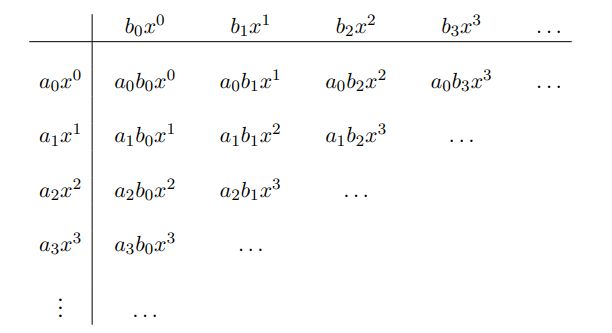
\includegraphics[scale=.5]{Convolution.PNG}
\label{fig:Conv}
\end{figure*}

Notice all the same powers of $x$ lie on the bottom left to top right diagonals. Notice how the subscripts of the coefficients are behaving in the Convolution way, with their sum always equalling to the power of $x$, this means the product of two infinite Polynomials $A(x)B(x)=C(x)$ will make

\begin{equation*}
    C(x)=\sum_{n=0}^{\infty} c_n x^n,
\end{equation*}

with $c_n=\sum_{k=0}^n a_{k}b_{n-k}=a_0b_n+a_1b_{n-1}+\ldots+a_{n-1}b_1+a_nb_0$. Notice again the $k$ and $n-k$ addition relationship shows up here as well. There is more to the study of Discrete Convolutions, however this is just enough for us to sense what a Continuous version of a Convolution will do and the Continuous one is the one we will need for Laplace study. Here is the convolution of two series now stated as one line.

\begin{equation*}
    \left(\sum_{n=0}^{\infty} a_n x^n\right)\left(\sum_{n=0}^{\infty} b_n x^n\right)=\sum_{n=0}^{\infty} \left[\sum_{k=0}^n a_{k}b_{n-k}\right] x^n.
\end{equation*}

\subsection{Convolution Integral}

Now that we have a sense of a Discrete Convolution. We can motivate the Continuous Convolution definition. Consider if instead of the 1 incremental in the addition problem like we did above with

\begin{equation*}
    5+0, \qquad 4+1, \qquad 3+2, \qquad 2+3, \qquad 3+2, \qquad 1+4, \qquad \text{ and } \qquad 0+5.
\end{equation*}

What if instead we instead change by .5 to get

\begin{equation*}
    5+0, \qquad 4.5+.5, \qquad 4+1, \qquad 3.5+1.5, \qquad 3+2, \qquad  \ldots
\end{equation*}

Even more granular we change by .01 and cycle through all the options

\begin{equation*}
    5+0, \qquad 4.99+.01, \qquad 4.98+.02, \qquad 4.97+.03, \qquad 4.96+.04, \qquad \ldots
\end{equation*}

Think of these as being inputs for an $a_k \cdot b_{n-k}$. Speaking of these in order to transition to continuous, the letters here are suggestive of being series which is inherently discrete, we shall rename them to $f_k$ and $g_{n-k}$. Also noting that the subscript is really just a way of condensing notation to make it easier to read, it really has the exact same effect as writing it in a function form of $f(k)$ and $g(n-k)$. Now consider if we continued this refining processes of what to plug into $k$ and $n-k$ so that $n=5$, however in order to get to continuous concepts, we will take the limit of this incremental as $k\rightarrow0$. Also, to stray away from letters that suggest discrete values, we rename them $n=t$ and $k=u$, now realize we are plugging in all possible positive real values into a $f(u)$ and $g(t-u)$. Recall since we kept $n$ constant we will keep $t$ constant as well likewise the $k$ changed so that changes $u$ along with the sum as well. Now long story short, with the limit making $u\rightarrow0$ and the sigma as part of the Convolution, we essentially set up a Riemann sum and the Sigma can turn into an integral sign now. Now motivating the Convolution Integral to be defined as

\begin{equation*}
    f(t) \ast g(t) = \int_{0}^{t} f(u)g(t-u) du.
\end{equation*}

With this definition now motivated, we will now see an example of this in action, consider the Convolution of $f(t)=t^2$ and $g(t)=t$ making

\begin{equation*}
    t^2 \ast t = \int_{0}^{t} u^2\cdot(t-u) du = \int_{0}^{t} u^2t-u^3 du = \left[\frac{u^3t}{3}-\frac{u^4}{4} \right]_{0}^{t} = \frac{t^4}{3}-\frac{t^4}{4}=\frac{t^4}{12}.
\end{equation*}

The applications for Convolutions are interesting, it will happen in Finance, Environmental Science, Chemistry, Physics, the discrete forms also applies in Probability Theory, Discrete Math, and Computer Science. A few examples like a continuously compounding interest while someone continuously withdraws from from the bank account would make a Convolution. Say you dump a radioactive isotope in a pile, we know that they decay at a rate proportional to their mass, but if we continuously add more of the isotope to the pile as a byproduct of some process the size of that pile will get modeled by a Convolution. For us we will stick to the Math of the Continuous Convolution instead of the modeling of it.

\subsection{Laplace and Convolution}

\subsubsection{Motivation}

Now that the Convolution is introduced, we see what good it is in the Laplace Transform and Differential Equation sense. We first make a callback to a few previous calculations we made in Laplace Transforms, first a property of Linearity $\lp[cf(t)]=c\lp[f(t)]$, the exponential input shift $\lp[e^{at}f(t)]=F(s-a)$ with $s-a>0$, and also a follow up calculation in the polynomial section $\lp[t^nf(t)]=(-1)^nF^{(n)}(s)$. These are examples of two functions being multiplied together to make a new Laplace entry. This leads to the natural curiosity, is there a general formula for 

\begin{equation*}
\lp[f(t)\cdot g(t)] = ?
\end{equation*}

The answer is there is not a nice general formula for this and it is proven there will never be one. However another wonder is in the inverse land of Laplace Transform, say we have two functions multiplied together and we are trying to find the inverse Laplace Transform of them. Is there a nice general formula that will find

\begin{equation*}
    \lp^{-1}[F(s)\cdot G(s)] = ?
\end{equation*}

The answer here is yes and it will involve the Convolution of their two input functions, $f(t)$ and $g(t)$ that Laplace to $F(s)$ and $G(s)$ respectively. We will note and prove the Laplace Transform property

\begin{equation*}
    \lp[f(t) \ast g(t)]=F(s)\cdot G(s).
\end{equation*}

\subsubsection{Convolution Theorem Proof}

We will start with the definition but we will weirdly prove this equation from right to left. Note that $F(s)=\int_0^{\infty} f(u) e^{-su} du$ and $G(s)=\int_0^{\infty} g(v) e^{-sv} dv$. Thus we start with

\begin{align*}
    F(s)\cdot G(s) &= \int_0^{\infty} f(u) e^{-su} du \cdot \int_0^{\infty} g(v) e^{-sv} dv \\
    &= \int_0^{\infty} \int_0^{\infty} f(u)g(v)e^{-s(u+v)}dudv.
\end{align*}

Note we are now in another Multivariable  Calculus Double Integral. Here we will do a change of variables with a Jacobian. We start with $t=u+v$ and $u=u$. The Jacobian makes a change of $dudv=\left|\frac{\partial(u,v)}{\partial(u,t)}\right|dudt$. Now recall that with $u=u$ and $v=t-u$, we execute the Jacobian determinant

\begin{equation*}
    \frac{\partial(u,v)}{\partial(u,t)}=\begin{bmatrix} \frac{\partial u}{\partial u} & \frac{\partial v}{\partial u} \\ \frac{\partial u}{\partial t} & \frac{\partial v}{\partial t} \end{bmatrix} = \begin{bmatrix} 1 & 0 \\ -1 & 1 \end{bmatrix}.
\end{equation*}

Now take the determinant of that matrix to get $(1)(1)-(-1)(0)=1$. Making no change so we have a seamless $dudv=dudt$. Now consider the limits changing. Our initial limits $\int_0^{\infty} \int_0^{\infty} f(t)g(t)e^{-s(u+v)}dudv$ mean that we are covering the entire first quadrant of the graph, also we integrate with $u$ then $v$, so we consider $u$ varies and $t$ is held fixed, since $t=u+v$, that means $u+v$ is a constant, and $u$ varies, this makes line segments on the first quadrant of the $(u,v)$ graph where the lines are decreasing linear lines entering on the vertical $v$ axis at $u=0$ and leaving the first quadrant on the horizontal $u$ axis at $v=0$, aka $u=t$. To cover the first quadrant, we need these parallel lines to hit at the origin, that will happen when $t=0$, then the diagonal line needs to cover the first quadrant making $t\rightarrow\infty$, that makes the new limits of $\int_0^{\infty} \int_0^{t}dudt$. Finishing off the change of variables, we see that

\begin{align*}
    F(s)\cdot G(s) = \int_0^{\infty} \int_0^{t} f(t)g(t-u)e^{-st}dudt \\
    F(s)\cdot G(s) = \int_0^{\infty} \left[\int_0^{t} f(t)g(t-u)du\right] e^{-st}dt \\
    F(s)\cdot G(s) = \int_0^{\infty} [f(t) \ast g(t)]e^{-st}dt \\
    F(s)\cdot G(s) = \lp[f(t) \ast g(t)].
\end{align*}

This proves the Convolution Theorem in Laplace Transforms.

\subsubsection{Example}

Consider a useful example of the now proven property, $\lp[f(t) \ast g(t)]=F(s)\cdot G(s)$. We will show a clever use for it, consider our previous example of $t^2 \ast t = \frac{t^4}{12}$. We will use this Laplace Transform of Convolution to calculate this same result quicker and without using the Convolution definition. We use our table entries to see that, $\lp[t^2]=\frac{2}{s^3}$ and $\lp[t]=\frac{1}{s^2}$, realize this makes

\begin{equation*}
    \lp[t^2 \ast t] = \frac{2}{s^3}\frac{1}{s^2}=\frac{2}{s^5}
\end{equation*}

Notice that if we take the inverse Laplace Transform to both sides of $\lp[t^2 \ast t] = \frac{2}{s^5}$, we get that $\lp^{-1}(\lp[t^2 \ast t]) = \lp^{-1}\left(\frac{2}{s^5}\right)$, or $t^2 \ast t=\lp^{-1}\left(\frac{2}{s^5}\right)$, so without using the definition of the Convolution we can still calculate the Convolution of $t^2$ and $t$, by just taking the Laplace Transform of each, multiplying them together, then take the inverse of that product. Realize that since $\frac{t^4}{12}$ has a Laplace Transform of $\frac{1}{12}\frac{4!}{s^5}=\frac{2}{s^5}$, we do get the same answer, $t^2 \ast t = \frac{t^4}{12}$, yet again.

\subsection{Properties of Convolution}

Here we will see the basic properties of Convolution which we can now prove them all since we have the Convolution Theorem Laplace trick now. We will start with the properties that only need the Convolution Integral Definition first, then show the properties that use the Laplace Trick.

\subsubsection{One Not Identity Element}

To begin we point out a basic idea in higher mathematics, the concept of identity elements. when we add a number like $a+0=a$, note that any number other than zero would make $a$ change into sometime else, but zero here let $a$ keep its identity after the addition, hence why mathematicians call these identity elements. Doing the same thing with $a\cdot0=0$, we see zero is not the multiplicative identity since $a$ did not retain its identity after the multiplication. However $a\cdot1=a$ does work so that means $1$ is the multiplicative identity. It seems like a trivial concept, that most things in life won't change if we multiply by 1 or add by zero. However some may have seen things like the concept of the identity matrix for matrix multiplication. If we say want a 2x2 matrix $I$ that multiplies with another 2x2 matrix $A$, such that $A\cdot I = A$, some may know the answer to the matrix that will retains $A$'s identity is 

\begin{equation*}
    I=\begin{bmatrix}
  1 & 0  \\
  0 & 1
 \end{bmatrix}.
\end{equation*}

if they were asked some people without experience in matrices to guess without calculating what the Identity will be they might think it is a matrix of all $1$ entries. A first lesson for some that identity elements will not always be a simple 1 or 0 number. It is hard to imagine those not being identity elements. However applying the Convolution Integral we will see that

\begin{equation*}
    f(t) \ast 1 = \int_{0}^{t} f(u) du=F(t)-F(0).
\end{equation*}

This is not retaining $f(t)$'s identity. Therefore the function $g(t)=1$ is not the Convolution's Identity element, a first big shocker of the Convolution not behaving like Multiplication. In a much later section we will introduce the function that will become the Convolution's identity element. \\

\subsubsection{Zero Function}

On another note,

\begin{equation*}
    f(t) \ast 0 = \int_{0}^{t} f(u)\cdot 0 du=0.
\end{equation*}

In that sense, the zero acts in the same way it does when in multiplication.

\subsubsection{Scalar Multiplication}

One more with the definition. Consider a constant $a$ multiplying with the Convolution output

\begin{equation*}
    a[f(t) \ast g(t)] = [af(t)] \ast g(t).
\end{equation*}

So by definition we see $a[f(t) \ast g(t)]=a\int_{0}^{t} f(u)\cdot g(t-u) du =\int_{0}^{t} [af(u)]\cdot g(t-u) du = [af(t)] \ast g(t)$. A simple proof here. This we name it the Associative Property with Scalar Multiplication.

\subsubsection{Commutative Property}

Now we look into properties that use the Laplace Transform Convolution Theorem, we can prove these properties quite easily relative to trying to prove them with only the integral definition. We start with considering two Laplace Transforms

\begin{equation*}
    \lp[f(t)\ast g(t)]=F(s)\cdot G(s),
\end{equation*}

then also

\begin{equation*}
    \lp[g(t)\ast f(t)]=G(s)\cdot F(s).
\end{equation*}

Since multiplication is Commutative making $G(s)F(s)=F(s)G(s)$ and we have a uniqueness theorem for Laplace Transforms, that must mean that $f(t) \ast g(t)=g(t) \ast f(t)$. Seeing the definition again, $f(t) \ast g(t) = \int_{0}^{t} f(u)g(t-u) du$, naturally it is tempting to think it would not be Commutative since the definition does not seem to treat the functions the same. However just because the formula looks asymmetrical is not a proof it is not Commutative, but our argument is a proof that it is Commutative. \\

Another way to try to wrestle with the counter-intuitiveness here, consider we try Commutative with the Binomial Theorem, consider if

\begin{equation*}
    (x+y)^n = \sum_{r=0}^{n} \binom{n}{r} x^{n-r}y^r = \sum_{r=0}^{n} \binom{n}{r} y^{n-r}x^r.
\end{equation*}

Also another intuition for Commutative is to try it with a small example for the Binomial Theorem, like $n=3$, we see the first form using $(x+y)^n = \sum_{r=0}^{n} \binom{n}{r} x^{n-r}y^r$, gets us $x^3+3x^2y+3xy^2+3y^3$. Now try the new looking second form of $(x+y)^n = \sum_{r=0}^{n} \binom{n}{r} y^{n-r}x^r$, it write out as $y^3+3y^2x+3yx^2+x^3$. It writes the same expression just arranged in the opposite order. This will also translate to the integral version when we think about it, the only thing different is the incremental is infinitesimal now instead of changing by 1 each time. \\

\subsubsection{Associative Property}

Next up we will prove the associative property, recall the basic associative property we are aware up like $(a+b)+c=a+(b+c)$, or $(a\cdot b) \cdot c = a \cdot (b \cdot c)$. We will see that we can prove that for Convolutions

\begin{equation*}
    (f(t) \ast g(t)) \ast h(t) = f(t) \ast (g(t) \ast h(t)).
\end{equation*}

The definition would take forever however. Note that since $\lp[a(t) \ast b(t)]=\lp[a(t)]\lp[b(t)]$, we call the expression in parenthesis and treat it like a single function so that

\begin{align*}
    \lp[(f(t) \ast g(t)) \ast h(t)] &= \lp[f(t) \ast g(t)]\lp[h(t)] \\
    &= \lp[f(t)]\lp[g(t)]\lp[h(t)] \\
    &=F(s)G(s)H(s).
\end{align*}

Now trying the same with the other side

\begin{align*}
    \lp[f(t) \ast (g(t) \ast h(t))] &= \lp[f(t)] \lp[g(t) \ast h(t)] \\
    &= \lp[f(t)]\lp[g(t)]\lp[h(t)] \\
    &=F(s)G(s)H(s).
\end{align*}

With them both being the same transform and by uniqueness theorem again we can say this associative property is true.

\subsubsection{Distributive Property}

Now let's consider a distributive property. We claim that

\begin{equation*}
    f(t) \ast (g_1(t)+g_2(t)) = f(t) \ast g_1(t) + f(t) \ast g_2(t).
\end{equation*}

Using Laplace again, we go get the left side
\begin{align*}
    \lp[f(t) \ast (g_1(t)+g_2(t))] &= \lp[f(t)] \cdot \lp[g_1(t)+g_2(t)] \\
     &= F(s) \cdot (\lp[g_1(t)]+\lp[g_2(t)]) = F(s) \cdot (G_1(s)+G_2(s)).
\end{align*}

Also the right side makes
\begin{equation*}
    \lp[f(t) \ast g_1(t) + f(t) \ast g_2(t)] = \lp[f(t) \ast g_1(t)] + \lp[f(t) \ast g_2(t)] = F(s)G_1(s)+F(s)G_2(s).
\end{equation*}

However since multiplication over addition has a distributive property, we know that $F(s)\cdot [G_1(s)+G_2(s)]=F(s)G_1(s)+F(s)G_2(s)$. Thus the transforms are the same and by the uniqueness property again we get to conclude that the Distributive Property of Convolution is officially a thing.

\subsubsection{Convolution One's Self}

Something else that happens in multiplication is the fact that $f(t)\cdot f(t)=f(t)^2\geq0$ for any value of $t$. So it may be tempting to think that $f(t) \ast f(t)$ will also be a non negative function that comes out. However we will calculate an example where that is not the case. Consider $f(t)=sin(t)$ to show this. We will use Laplace to calculate $sin(t) \ast sin(t)$ which is

\begin{equation*}
    \lp[sin(t) \ast sin(t)]=\frac{1}{s^2+1}\frac{1}{s^2+1}=\frac{1}{(s^2+1)^2}.
\end{equation*}

Now we need to take the inverse Laplace to find our Convolution back. Consider in our Laplace of polynomial work we derived that $\lp[t^n \cdot f(t)]=(-1)^n \frac{d^n}{ds^n}F(s)$, especially when we are getting squares of simpler transforms this entry can be useful, notably our example of this formula in that section was calculating $\lp[t \cdot cos(at)]=\frac{s^2-a^2}{(s^2+a^2)^2}$. We will continue with this property to make another notable transform that might be worthy enough for your own personal table. Consider

\begin{align*}
    \lp[sin(at) - at \cdot cos(at)] &= \frac{a}{s^2+a^2}-a\frac{s^2-a^2}{(s^2+a^2)^2} \\
    &= \frac{a(s^2+a^2)}{(s^2+a^2)^2}-\frac{a(s^2-a^2)}{(s^2+a^2)^2} \\
    &=\frac{as^2+a^3-(as^2-a^3)}{(s^2+a^2)^2} \\
    &=\frac{2a^3}{(s^2+a^2)^2}.
\end{align*}

Back to our inverse problem using what we just got with $a=1$, makes $\frac{2}{(s^2+1)^2}$ getting us really close to what we need to find. We will manipulate our expression a little to make $\frac{1}{(s^2+1)^2}=\frac{1}{2}\frac{2}{(s^2+1)^2}$. Thus our final answer is $\frac{1}{2}[sin(t)-tcost(t)]$. That means

\begin{equation*}
    sin(t) \ast sin(t) = \frac{1}{2}[sin(t)-tcost(t)].
\end{equation*}

Notice that this will not always be bigger than zero for every value of $t$, for example $t=2\pi$ makes $\frac{1}{2}[sin(2\pi)-2\pi cost(2\pi)]=-\pi$. Thus we do not get to have a guaranteed positive squared property in Convolution.

\subsection{The Beta Function with Gamma Connection}

Here we will introduce yet another function, given what we covered with Gamma Function and Convolution, we will be able to handle its complexity and annoyance now. It is defined as

\begin{equation*}
    \beta(a,b) = \int_{0}^{1} (1-x)^{a-1}(x)^{b-1} dx.
\end{equation*}

This function has some interesting applications, there is a distribution in Statistics called the Beta Distribution, take too much to talk about how a real life probability situation will be a Beta Distribution, however at the end of this section we will happen to see the formula for the Beta Distribution in our work. It gets used in Quantum Mechanics and other physics as well. There are multitudes of methods that work to calculate this integral. The first thought of trying integration by parts does not bode well when attempted. In physics they will do many U-substitutions, Trig Substitutions and other standard  Calculus techniques to turn this into different forms to convince us of seemingly different looking situations that can all be modeled by this function. In Statistics there are clever integral techniques to shortcut this calculation. One is a technique called Bayes Billiards, were we literally calculate the integral by telling a probability story involving balls thrown on a billiard table. Another is to use the Gamma Function which is related to the Gamma Distribution, once there we create a Multivariable Distribution, then do a change of variable with Jacobian technique, then out of the blue the answer to the Beta integral happens to show up in a seemingly off topic problem. \\

The technique we will use to calculate this integral is by using Laplace Transforms and the Convolution Theorem. The answer to this integral is actually in terms of Gamma Functions, hence our title claiming there is a Gamma connection. It will be

\begin{equation*}
    \beta(a,b) = \int_{0}^{1} (1-x)^{a-1}(x)^{b-1} dx = \frac{\Gamma(a)\Gamma(b)}{\Gamma(a+b)}.
\end{equation*}

We will get there by starting with known definitions, and up the complexity until we obtain the above, also since we are in Laplace we will do this using $x=t$ since we usually been using $t$'s in Laplace transforms. We first start with our Laplace of Gamma table entry $\lp[t^{\alpha-1}]=\frac{\Gamma(\alpha)}{s^{\alpha}}$, multiply the denominator to the other side and rename it with $a$ and $b$ instead gives us

\begin{equation*}
    \Gamma(a)=s^a\lp[t^{a-1}] \qquad \text{and} \qquad \Gamma(b)=s^b\lp[t^{b-1}].
\end{equation*}

Multiply them together to get

\begin{equation*}
    \Gamma(a)\Gamma(b)=s^{a+b} \cdot \lp[t^{a-1}] \cdot \lp[t^{b-1}].
\end{equation*}

Consider dividing the $s$ term and then taking the Inverse Laplace Transform of both sides of this equation.

\begin{align*}
    \frac{\Gamma(a)\Gamma(b)}{s^{a+b}} &= \lp[t^{a-1}] \cdot \lp[t^{b-1}] \\
    \lp^{-1}\left[\frac{\Gamma(a)\Gamma(b)}{s^{a+b}}\right] &= \lp^{-1}\left[\lp[t^{a-1}] \cdot \lp[t^{b-1}]\right].
\end{align*}

The interesting part of the derivation is here, we have on the right side a product of two Laplace transforms that we are trying to find the inverse of, that is in essence what the Convolution Theorem accomplishes. Recall the entry, $\lp[f(t) \ast g(t)] = F(s)\cdot G(s)$. We will then switch notation, and take the inverse Laplace of both sides to get

\begin{align*}
    F(s)\cdot G(s) &= \lp[f(t) \ast g(t)] \\
    \lp[f(t)]\cdot\lp[g(t)] &= \lp[f(t) \ast g(t)] \\
    \lp^{-1}(\lp[f(t)]\cdot\lp[g(t)])&=\lp^{-1}(\lp[f(t) \ast g(t)]) \\
    \lp^{-1}(\lp[f(t)]\cdot\lp[g(t)])&=f(t) \ast g(t).
\end{align*}

That means for us, we can use this to change our right hand side with $f(t)=t^{a-1}$ and $g(t)=t^{b-1}$. We are now at

\begin{equation*}
    \lp^{-1}\left[\frac{\Gamma(a)\Gamma(b)}{s^{a+b}}\right] = t^{a-1} \ast t^{b-1}.
\end{equation*}

Recall the definition of Convolution is $f(t) \ast g(t) = \int_{0}^{t} f(u)g(t-u) du$. Also since it is Commutative, we will actually calculate $t^{b-1} \ast t^{a-1}$ instead to get

\begin{equation*}
    t^{b-1} \ast t^{a-1} = \int_{0}^{t} (u)^{b-1}\cdot(t-u)^{a-1} du = \int_{0}^{t} (t-u)^{a-1} \cdot (u)^{b-1} du.
\end{equation*}

Then we we will perform a substitution $v=\frac{u}{t}$ or $u=tv$. That makes $\frac{dv}{du}=\frac{1}{t}$, or $du = tdv$. Also for adjusting the limits, when $u=0$, that makes $v=0$, then when $u=t$, that makes $v=\frac{t}{t}=1$. Executing the substitution we begin to see the Beta function form on the right.

\begin{align*}
    \int_{0}^{t} (t-u)^{a-1} \cdot (u)^{b-1} du &= \int_{0}^{1} (t-tv)^{a-1} \cdot (tv)^{b-1}\cdot t dv \\
    &= t\int_{0}^{1} (t)^{a-1}(1-v)^{a-1}(t)^{b-1}(v)^{b-1} dv \\
    &=t^{a+b-1} \int_{0}^{1} (1-v)^{a-1}(v)^{b-1} dv.
\end{align*}

Back to big picture. We made some progress on the right hand side of $\lp^{-1}\left[\frac{\Gamma(a)\Gamma(b)}{s^{a+b}}\right] = t^{a-1} \ast t^{b-1}$ to be updated to

\begin{equation*}
    \lp^{-1}\left[\frac{\Gamma(a)\Gamma(b)}{s^{a+b}}\right] = t^{a+b-1} \int_{0}^{1} (1-v)^{a-1}(v)^{b-1} dv.
\end{equation*}

First renaming the dummy variable $v$ to $x$ and swapping, we are now at

\begin{equation*}
    t^{a+b-1} \cdot \int_{0}^{1} (1-x)^{a-1}x^{b-1} dx=\lp^{-1}\left[\frac{\Gamma(a)\Gamma(b)}{s^{a+b}}\right].
\end{equation*}

Next is to address the extra $t^{a+b-1}$ term. To make something different about it, we will take the Laplace transform of both sides, cancelling the right side, the Integral is considered a constant since it is not dependent on $t$, so it can get pulled out of the transform, this makes

\begin{align*}
    \lp\left(t^{a+b-1} \cdot \int_{0}^{1} (1-x)^{a-1}x^{b-1} dx\right) &= \lp(\lp^{-1}\left[\frac{\Gamma(a)\Gamma(b)}{s^{a+b}}\right]) \\
    \lp[t^{a+b-1}] \cdot \int_{0}^{1} (1-x)^{a-1}x^{b-1} dx &= \frac{\Gamma(a)\Gamma(b)}{s^{a+b}}.
\end{align*}

At this point it is now $\lp[t^{a+b-1}]$ we have to address, and we have a nice way to deal with it. Since we have the Laplace involving Gamma as $\lp[t^{\alpha-1}]=\frac{\Gamma(\alpha)}{s^{\alpha}}$, we replace $\alpha=a+b$ to get

\begin{equation*}
    \lp[t^{a+b-1}]=\frac{\Gamma(a+b)}{s^{a+b}}.
\end{equation*}

Substitute this into our current progress, multiply to cancel out $s^{a+b}$ and we will finally have our Beta to Gamma equation

\begin{align*}
    \lp[t^{a+b-1}] \cdot \int_{0}^{1} (1-x)^{a-1}x^{b-1} dx &= \frac{\Gamma(a)\Gamma(b)}{s^{a+b}} \\
    \frac{\Gamma(a+b)}{s^{a+b}} \cdot \int_{0}^{1} (1-x)^{a-1}x^{b-1} dx &= \frac{\Gamma(a)\Gamma(b)}{s^{a+b}} \\
    \Gamma(a+b) \cdot \int_{0}^{1} (1-x)^{a-1}x^{b-1} dx &= \Gamma(a)\Gamma(b) \\
    \int_{0}^{1} (1-x)^{a-1}x^{b-1} dx &= \frac{\Gamma(a)\Gamma(b)}{\Gamma(a+b)}.
\end{align*}

This completes the proof calculating the integral as well as we are going to get. \\

For a small example, realize if the integral has $a=6$ and $b=8$, then with Gamma properties that makes

\begin{equation*}
    \int_{0}^{1} (1-x)^{5}x^{7} dx = \frac{\Gamma(6)\Gamma(8)}{\Gamma(14)} = \frac{5!7!}{13!} = \frac{1}{10,296}.
\end{equation*}

So now we can solve what would be very tedious integrals quite quickly now. Historically this calculation of Gamma and Beta happened pretty early on in the beginning of Calculus's life. Leonhard Euler(1707-1783) was the one that first studied the Beta and Gamma functions. In light of that, some call the Beta function the Euler Integral of the First Kind and the Gamma the Euler Integral of the Second Kind. \\

Another basic follow up, aka a Corollary, is to realize we can multiply by the the reciprocal on the right and tuck it into the integral making it look like

\begin{equation*}
    \int_{0}^{1} \frac{\Gamma(a+b)}{\Gamma(a)\Gamma(b)}(1-x)^{a-1}x^{b-1} dx = 1.
\end{equation*}

Those with Statistics knowledge realize this helps justify that this integrand is a Probability Density Function. Thus the Beta distribution is listed as the integrand of this with possible values of $x$ being between 0 and 1.

\subsection{Solving Equations with a Convolution}

Consider solving the following Differential Equation,

\begin{equation*}
    4y"+y=g(t), \qquad y(0)=3 \qquad y'(0)=-7.
\end{equation*}

Note that we are solving for an unknown function for an Inhomogenous equation, showing that Laplace Transform is powerful enough to solve it anyway, Variation of Parameters would need to know what $g(t)$ in order to begin guessing what to do with it. For the sake of naming it we will call $g(t)$ or any non zero function on the right side the Forcing Function. Since it is usually in application, acting as the outside force of a physical system. \\

We start with the Usual Laplace Transform of both sides, note that $\lp[g(t)]=G(s)$,

\begin{align*}
    4(s^2\hugey-sy(0)-y'(0))+\hugey &=G(s) \\
    (4s^2+1)\hugey-12s+28 &=G(s) \\
\end{align*}

Now solve for $\hugey$,

\begin{align*}
    (4s^2+1)\hugey&=G(s)+12s-28 \\
    \hugey &= \frac{12s-28}{4(s^2+\frac{1}{4})} + \frac{G(s)}{4(s^2+\frac{1}{4})}.
\end{align*}

We factored out the 4 in the denominator for anticipating it will be easier to match up the form we need for the inverse Transforms. A little more rearranging to make that happen gets

\begin{align*}
    \hugey &= \frac{12s-28}{4(s^2+\frac{1}{4})} + \frac{G(s)}{4(s^2+\frac{1}{4})} \\
    &= \frac{3s}{s^2+\frac{1}{4}}-\frac{7\frac{2}{2}}{s^2+\frac{1}{4}} + \frac{1}{4}G(s)\frac{\frac{2}{2}}{s^2+\frac{1}{4}}.
\end{align*}

Now, the first two terms are typical inverse Transforms. They are $3cos\left(\frac{t}{2}\right)$, since $\lp[3cos\left(\frac{t}{2}\right)]=\frac{12s}{4s^2+1}$ and the second term inverse is $14sin\left(\frac{t}{2}\right)$ since $\lp[14sin\left(\frac{t}{2}\right)]=\frac{28}{4s^2+1}$ The last term will need a Convolution integral on the last term, since it is two functions in Laplace Transform Land being multiplied together and the inverse of that is the Convolution of their individual inverses. The two functions for this Convolution will be

\begin{equation*}
    g(t) \qquad \text{and} \qquad f(t)=2sin\left(\frac{t}{2}\right).
\end{equation*}

Check to make sure, Laplace of $g(t)$ makes $G(s)$ and Laplace of $2sin\left(\frac{t}{2}\right)$ makes $\frac{4}{4s^2+1}$, with a little arranging will meet as needed for the last term. Finishing the job, our full inverse Transform gives us,

\begin{equation*}
    y(t)=3cos\left(\frac{t}{2}\right)-14sin\left(\frac{t}{2}\right)+\frac{1}{2}\int_{0}^{t}sin\left(\frac{\tau}{2}\right)g(t-\tau) d\tau.
\end{equation*}

So, once we decide on a $g(t)$ all we need to do is an integral and we'll have the solution. Clever, Variation of Parameters cannot go this far.

\subsection{Transfer, Impulse Response, and Integral Equation}

We will solve a differential equation again but this time we will really generalize the problem. Consider trying to solve

\begin{equation*}
    ay"+by'+cy=g(t) \qquad y(0)=y_0 \quad y'(0)=y'_0.
\end{equation*}

Now we do not just have an unknown right hand side $g(t)$ Forcing Function, but we also have parameters $a,b,c,y_0,y'_0$ in play being constants we do not know yet. This problem could even get more annoying if the left side of the differential equation did not have constant coefficients like ours has right now. For now we will solve this one, any of our other second order methods would only get part way there at best, Laplace can really take us further in these solves. We take Laplace of both sides

\begin{align*}
    as^2\hugey-asy(0)-ay'(0)+bs\hugey-by(0)+c\hugey &= G(s) \\
    (as^2+bs+c)\hugey - (as+b)y_0 - ay'_0 &= G(s).
\end{align*}

Remember our differential equation solution is a $y(t)$, its Laplace Transform is $\hugey$, so we solve for that.

\begin{align*}
    (as^2+bs+c)\hugey &= (as+b)y_0+ay'_0+G(s) \\
    \hugey &= \frac{(as+b)y_0+ay'_0}{(as^2+bs+c)}+\frac{G(s)}{(as^2+bs+c)}.
\end{align*}

Now we name some parts. Consider naming $\Phi(s)=\frac{(as+b)y_0+ay'_0}{(as^2+bs+c)}$, and $\Psi(s)=\frac{G(s)}{(as^2+bs+c)}$. This condenses what we have as

\begin{equation*}
    \hugey = \Phi(s)+\Psi(s).
\end{equation*}

then we can take the Inverse Laplace of both sides, where sticking to our usual upper and lowercase notation scheme, $\lp^{-1}[\Phi(s)]=\phi(t)$ and $\lp^{-1}[\Psi(s)]=\psi(t)$ making the solution look like

\begin{equation*}
    y(t) = \phi(t)+\psi(t).
\end{equation*}

Also a big observation, if we were to calculate it, we would find that $\phi(t)$ is the solution to a simpler initial value problem(IVP), we could Laplace transform the following to derive the same answer as $\lp^{-1}[\Phi(s)]=\phi(t)$

\begin{equation*}
    ay"+by'+cy=0 \qquad y(0)=y_0 \quad y'(0)=y'_0.
\end{equation*}

Also note $\psi(t)$ is the solution to this, again we could confirm it by taking the Laplace and solve. 

\begin{equation*}
    ay"+by'+cy=g(t) \qquad y(0)=0 \quad y'(0)=0
\end{equation*}

Notice the difference between the two. First IVP is homogeneous but keeping the initial values, the second IVP keeps $g(t)$ but zeros out the initial values. So once we are given the values of $a,b,c,y_0,y'_0$ to make a specific problem. We can stick it into $\Phi(s)$ and inverse Laplace solve it real quick. Then addressing $\Psi(s)$, we break down $\Psi(s)=H(s)G(s)$, where $H(s)=(as^2+bs+c)^{-1}$. This $H(s)$ will now be given the name the Transfer Function. Realize when we try to inverse $\Psi(s)$ we are instead trying to find $\lp^{-1}[H(s)G(s)]$, however that will turn into $h(t)\ast g(t)$ by the Convolution theorem. This is continuing our notation scheme $\lp^{-1}[H(s)]=h(t)$, and $\lp^{-1}[G(s)]=g(t)$. By definition of Convolution we now have the integral to find

\begin{equation*}
    \psi(t)=\lp^{-1}[H(s)G(s)] = \int_{0}^{t} h(t-\tau)g(t) d\tau.
\end{equation*}

We call the $h(t)$ in our Convolution the Impulse Response Function. Now our solution could also look like

\begin{equation*}
    y(t) = \phi(t)+\int_{0}^{t} h(t-\tau)g(t) d\tau.
\end{equation*}

So instead of solving a differential equation to find a solution to a problem, we can stick in our parameter values, calculate the functions to plug and solve this integral equation instead. This study can get deeper, a follow up study is to list example solutions of $y(t)$ and then solve variations of this equation to solve what types of functions would work and don't work, essentially it could be used to reverse engineer what solutions will have what kind of Differential Equations governing them. Sometimes derivatives will creep into these as well, making another term called integro-Differential Equations. We will not be looking into these.

\section{Unit Step Function}

\subsection{Basics}

\subsubsection{Definition}

Unit Step Function or the Heaviside function named after Oliver Heaviside (1850–1925). It is quite a utility function but quite simple looking. People tend to underestimate this function and concept though and get blindsided by some obscure concepts not really practiced. This will take a keen ability to sense and marry geometric graphical visuals with algebraic manipulations, something students may not do enough of in practice. Here is the definition

\begin{equation*}
    u(x)=\left\{
        \begin{array}{rl}
            1 &  x \geq 0  \\
            0 &  x < 0.
        \end{array}
    \right.
\end{equation*}

We will be self consistent with our notation system, be aware though there are many notation systems for this and what is about to come, some of which will conflict with each other from one classroom to the next. We can cheaply use the unit Step Function by realizing if we try to find some $u(c)$, when $c$ is a positive number it is an output of 1, negative it is an output of 0. Examples like $u(-6)=0$, and $u(\pi)=1$ will help us mentally calculate in the future. Visualizing it we get why it is called a Step Function, since it makes this graph.

\begin{figure*}[!htbp]
\centering
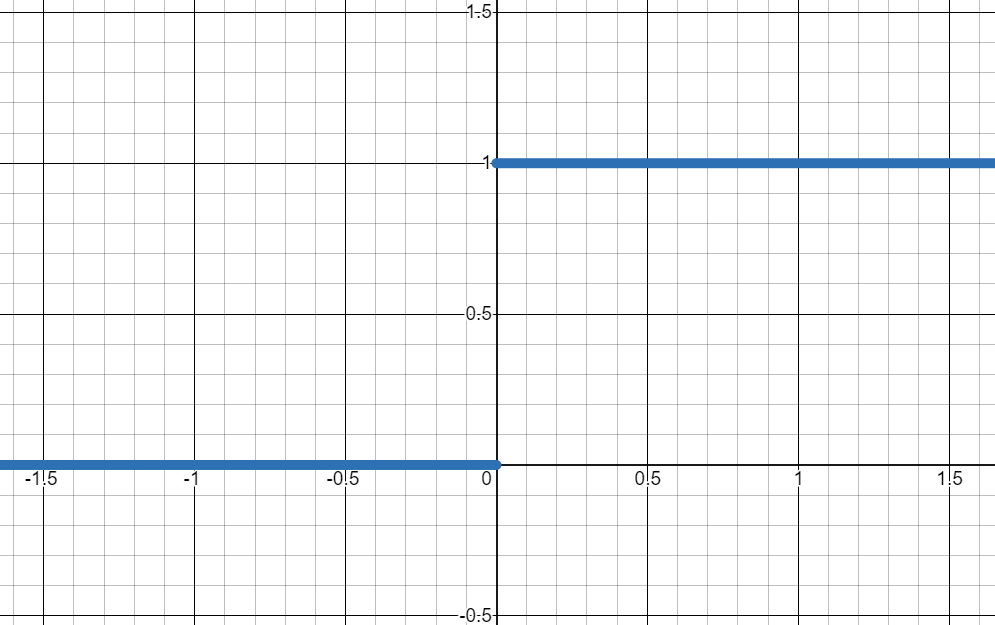
\includegraphics[scale=.4]{step.PNG}
\label{fig:hsf}
\end{figure*}

\subsubsection{Exercise 1}

Seems basic to start but now we consider exercises using this Step Function, there will be a lot of guesswork, the important part is not your initial guesses per say, it is your ability to check them and confirm your guess is right or if it is wrong to figure out why it is wrong so we can eventually be right. Consider trying to write out the following piece wise function using unit Step Functions. 

\begin{equation*}
    f_1(x)=\left\{
        \begin{array}{rl}
            1 &  x \geq 3  \\
            0 &  x < 3.
        \end{array}
    \right.
\end{equation*}

Eventually it will be up to you to mentally picture this

\begin{figure*}[!htbp]
\centering
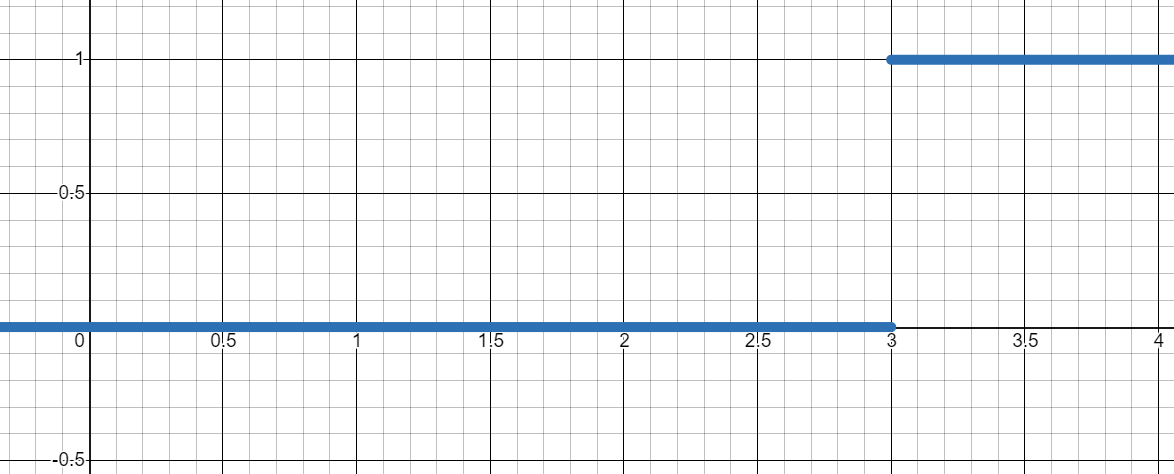
\includegraphics[scale=.4]{step1.PNG}
\label{fig:hsf1}
\end{figure*}

Visually speaking, this is taking our $u(x)$ and shifting the graph 3 units to the right. That means we can write it with the unit Step Function as $u(t-3)$. Try some values of $x$ and see if the output aligns with height of the graph in the picture, for example, if $x=2$, then we get $u(2-3)=u(-1)=0$, our picture some places will shorthand this by denoting it with a subscript, we will save the subscript notation for a different topic that those sources are not covering.

\subsubsection{Exercise 2}

Another exercise, again rewrite this with a unit Step Function. 

\begin{equation*}
    f_2(x)=\left\{
        \begin{array}{rl}
            4 &  x \geq 2  \\
            0 &  x < 2.
        \end{array}
    \right.
\end{equation*}

Again you should be picturing this in your head. 

\pagebreak

\begin{figure*}[!htbp]
\centering
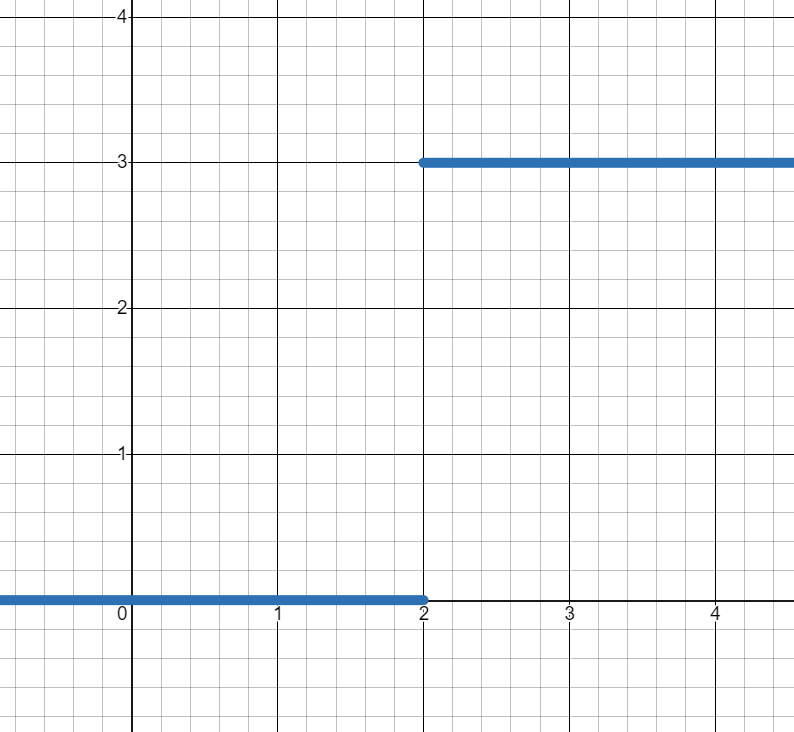
\includegraphics[scale=.4]{step2.PNG}
\label{fig:hsf2}
\end{figure*}

Now we describe it as a shift to the right by 2, so we can start with $u(x-2)$ but how do we account for the vertical change? It may be tempting to just guess $3+u(x-2)$, however plug in some values and see if it aligns with our graph. for example, when $x=1$ that means $3+u(1-2)=3+u(-1)=3+0=3$, wait the graph we have has their line at $0$ when $x=1$. Another example shows we are spot on the other piece, when $x=3$, then $3+u(3-2)=3+u(1)=3+1=4$, as shown on the graph. It is a conundrum, like solving a Rubik's cube, you want to put a color in a proper place on the cube without messing up another spot that is already in place. \\

This is where the art form of guessing and checking comes in, those that work with Rubik's cubes before know you might have to temporary move a piece from its correct spot to move something else. A new guess of $u(x-2)$ we can sense pretty quickly is incorrect, but check it anyway, the important part is not figuring out if your guess is incorrect but why it is incorrect. We have when $x=1$, then $u(1-2)=u(-1)=0$, as needed, however, $x=3$ makes $u(3-2)=u(1)=1$, but that value needs to output 3. It may seemed like we did not do any better progressing towards the solution with that guess, we just swapped which piece was correct. However a different vantage point may be the key to seeing an observation needed to solve it, from this outcome if we realize that we can multiply the output of $0$ and $1$ we currently got by 4, then we will get outputs of $0$ and $4$, meaning we should try to vertically stretch the function instead. We guess $4\cdot u(x-2)$ and see that $x=1$ makes $4\cdot u(1-2)=4\cdot u(-1)=4(0)=0$, and also say $x=3$ makes $4\cdot u(3-2)=4\cdot u(1)=4(1)=4$ as needed. This leads to the eventually correct guess. Eventually enough guesswork will lead to more intuition on what to guess and the process will move quicker with experience. \\

\subsubsection{Exercise 3: Box Function}

Consider finding in terms of Step Functions,

\begin{equation*}
    f_3(x)=\left\{
        \begin{array}{rl}
            0 & x < -3  \\
            1 & -3 \leq x < 1 \\
            0 & 1 \leq x. 
        \end{array}
    \right.
\end{equation*}

This makes a visual of

\begin{figure*}[!htbp]
\centering
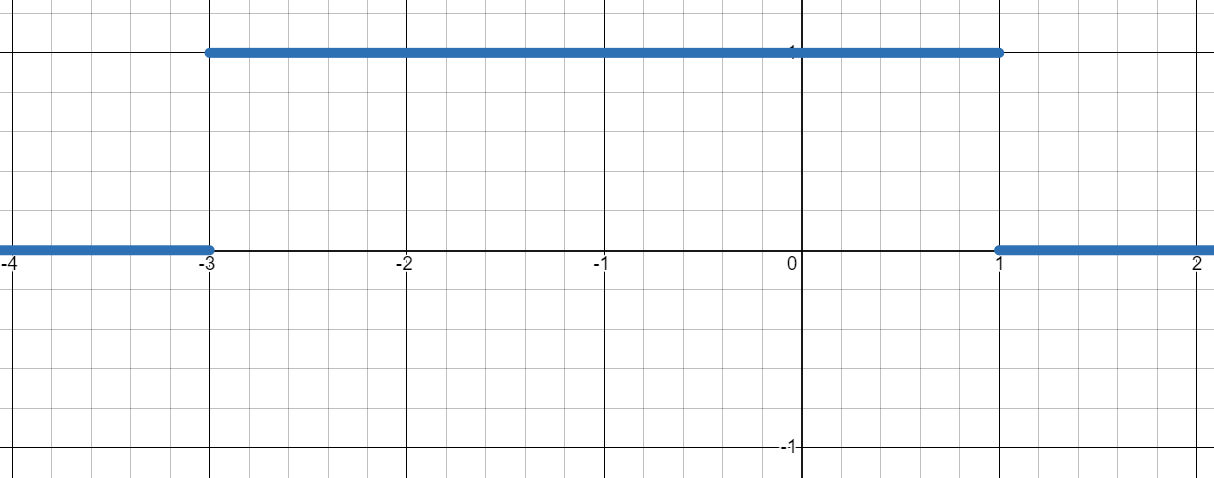
\includegraphics[scale=.4]{step3.PNG}
\label{fig:hsf3}
\end{figure*}

A first observation to make is we now have two jump discontinuities in this one, since the unit Step Function only has at most one no matter how we stretch, shrink, reflect, or translate the graph. We are going to need a second unit Step Function in our expression. To illustrate, consider a guess of say $u(x+3)$, when $x=-4$, we get $u(-4+3)=u(-1)=0$, which agrees with our graph, we also agree with $x=-2$ being $u(-2+3)=u(1)=1$ which also agrees. We may think we are done testing and call this right since that is what we did last time, but that is no guarantee. Trying out a third test point here we get $x=2$ makes $u(2+3)=u(5)=1$, however our graph says we should be at 0. By all means try three points or more on our previous examples if you are not convinced those are correct now, we assure that they are correct, but do not take our word for it. \\

So realize we need to make the graph jump down to 0, so at the very least we need a jump discontinuity at $x=1$, that leads us to think we will also need a $u(x-1)$ function in our expression as well. Guessing $u(x+3)-u(x-1)$ we see that there are 3 regions between the 2 jumps, we will test a point in each region to confirm they are correct. So with $x=-4$ we get $u(-4+3)-u(-4-1)=u(-1)-u(-5)=0-0=0$ as shown on the graph, also $x=0$ makes $u(0+3)-u(0-1)=u(3)-u(-1)=1-0=1$ also agreeing with the graph, then finally a $x=2$ makes $u(2+3)-u(2-1)=u(5)-u(1)=1-1=0$. Enough confirmation for us to think we may have a correct guess. \\

To generalize this graph we see here, since it looks like a box, people may call this a box function. To fully generalize this, consider a box with the jump up at $x=a$ and jump back down at $x=b$, then let's also say the height of the box generalizes from 1 that our problem had to an output of $c$ for us. We see that $c[u(t-a)-u(t-b)]$ will be what makes the box happen in general. We will be taking advantage of this general box function in the Dirac Delta Function section coming later.

\subsubsection{Exercise 4}

Now for an exercise fully generalizing the basic step concept, again consider finding in terms of $u$ functions,

\begin{equation*}
    f_4(x)=\left\{
        \begin{array}{rl}
            -4 &  x < 6  \\
            25 &  6 \leq x < 8 \\
            16 &  8 \leq x < 30 \\
            10 &  30 \leq x.
        \end{array}
    \right.
\end{equation*}

Without the graph this time, picture it in your head as we go, we have a leftmost piece of $-4$, since every unit Step Function is 0 to the left of their jump, that -4 will not happen with our Step Function, so we start our guess at -4. Now we consider the Step Functions from there, realize we have jumps at 6, 8 and 30. These 3 discontinuities means we will want to use 3 Step Functions of $u(x-6)$, $u(x-8)$ and $u(x-30)$ respectively. We will try building our guess from left to right, consider $-4+29u(x-6)$, to the left of $x=6$ we have the $u=0$ so we get the $-4$ as needed, to the right of $x=6$ we have $-4+29(1)=25$ constructing our second piece, now we need to make another jump at $x=8$, so we append to our guess of $-4+29u(x-6)-9u(x-8)$, again left of $x=6$ which is also left of $x=8$ makes $-4+29(0)-9(0)=-4$, then between 6 and 8 we get $-4+29(1)-9(0)=25$ as needed, then to the right of both 6 and 8 is $-4+29(1)-9(1)=16$. Now that we have a patternistic intuitive construct here, we can continue this line of thinking and also tack on $-4+29u(x-6)-9u(x-8)-6u(x-30)$ and be decently confident in it.

\subsubsection{Exercise 5}

It is one thing to make Step Function with it, but it also has more applications, consider the function will make the following piece wise 

\begin{align*}
    x^2\cdot u(x-2) = \left\{
        \begin{array}{cc}
            0 & x < -2  \\
            x^2 & -2 \leq x. 
        \end{array}
    \right.
\end{align*}

The graph of this makes

\pagebreak

\begin{figure*}[!htbp]
\centering
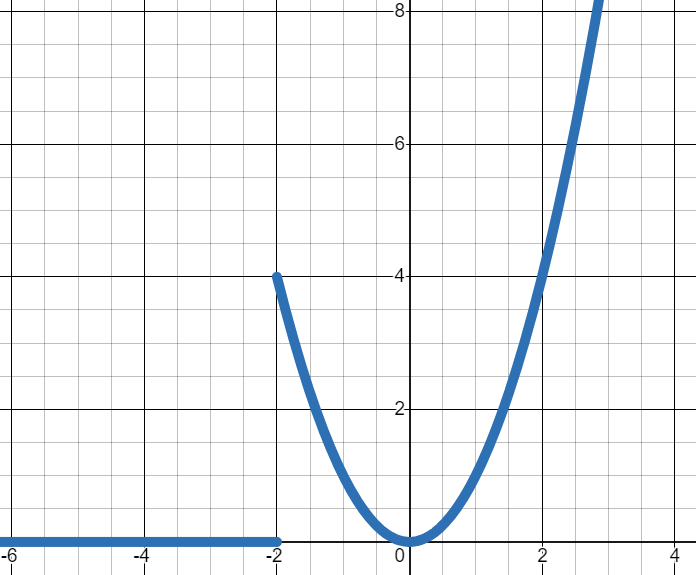
\includegraphics[scale=.5]{step4.PNG}
\label{fig:hsf4}
\end{figure*}

Notice how the unit Step Function basically truncates the $x^2$ graph at its discontinuity. We think a Step Function like as an on off switch to a music player essentially and the function is like a dial for adjusting the volume. Now we try to offer up another exercise, how can we write in terms of Step Functions, where we put in $x^2$ to the left of -2 and truncate the right side of the graph instead? 

\begin{figure*}[!htbp]
\centering
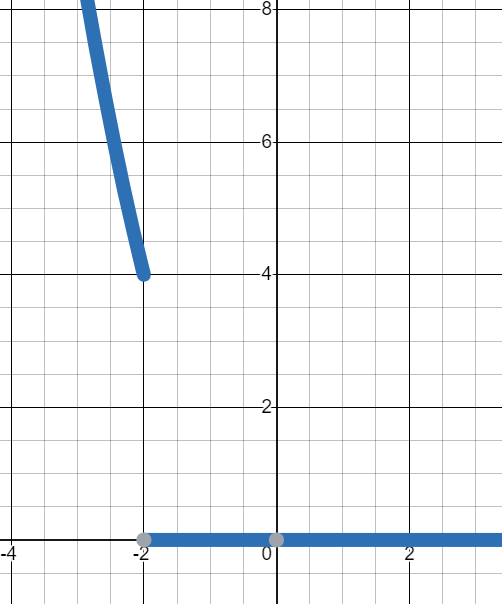
\includegraphics[scale=.5]{step5.PNG}
\label{fig:hsf5}
\end{figure*}

We essentially want to switch around the on off switch so to speak, so how do we make a Step Function that is 1 to the left and 0 to the right of its discontinuity? The answer is $1-u(x)$, realize left of 0, we have $1-(0)=1$ and right of zero we have $1-(1)=0$ as needed. Then we can shift this function to the left 2 units and get $1-u(x+2)$, now we multiply with the $x^2$ and get an answer of $x^2\cdot(1-u(x+2))$. \\

\subsection{Laplace and Step Functions}

\subsubsection{Laplace with Step}

We start with taking a Laplace Transform of the original $u(x)$, we get

\begin{equation*}
    \lp[u(t)]= \int_0^{\infty} u(t) e^{-st} dt=\int_0^{\infty} 1e^{-st} dt=\frac{1}{s} \qquad s>0.
\end{equation*}

Note how this is the same as $\lp[1]$, the bounds on the integral only care about values on the positive axis, so for the entire integral the unit Step Function will be 1. This was a hidden but now very apparent property of the Laplace Transform, it cannot handle functions that have negative valued inputs since the limits do not consider them. From the Laplace perspective, inputting 1 and $u(x)$ are the same thing to it. \\

This leads to the question, what really is $\lp^{-1}[u(t)]$? We were a little misleading when we first introduced the Inverse Laplace Transform saying there was a uniqueness theorem. In fact that Uniqueness theorem is still true, but only on the interval $[0,\infty)$, the function's negative inputs does not have to satisfy and infinitely many possibilities can happen. Once we have to deal with Jump discontinuities in solving Differential Equations, have the inverse be $\lp^{-1}(u(t))=1$ will no longer be good enough, even though it has been good enough up until now. At this point onward we define the Laplace Transform as $\lp[f(t)]=F(s)$, but now instead of $\lp^{-1}[F(s)]=f(t)$, in this new context we now define and force the negative values of the function to be zero, making it $\lp^{-1}[F(s)]=u(t)f(t)$. \\

\subsubsection{Laplacing Truncated Functions}

Now to investigate another question. Is there a way to translate a function left and right and write $\lp[f(t-a)]$ in terms of Laplacing some form of $f(t)$ to make it equivalent? The realization will come from the graphs.

\pagebreak

\begin{figure*}[!htbp]
\centering
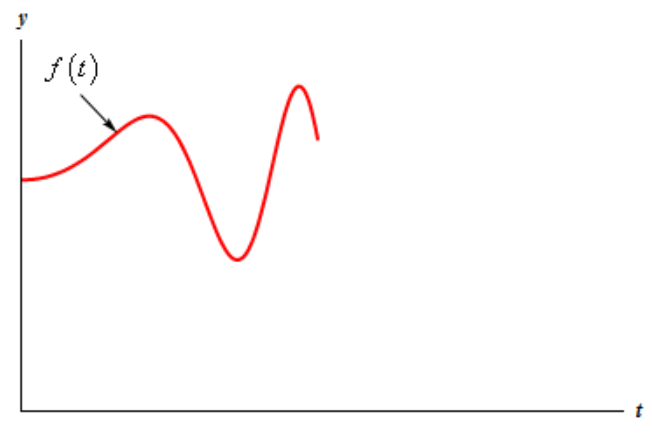
\includegraphics[scale=.5]{step6.PNG}
\label{fig:hsf6}
\end{figure*}

Note the function is cut off at $t=0$ for the negative values of $t$ we do not know what really happens with $y$ this is from the perspective of the Laplace Transform since its integration is from 0 to $\infty$. However realize once we shift the function to the right by $c$.

\begin{figure*}[!htbp]
\centering
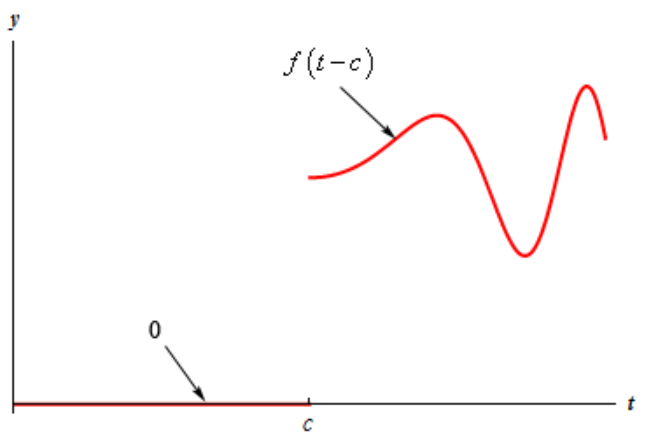
\includegraphics[scale=.5]{step7.PNG}
\label{fig:hsf7}
\end{figure*}

Now note to complete this function of $f(t-c)$ we would need to know the real outputs of $f(t)$ between the values of $-c<t<0$ before the unit Step Function turned off the function and made it zero. 

\subsubsection{The Correction}

However the Laplace Transform would not know what that is, making that information is lost once we take the Laplace Transform of a function, so there is no way to relate Laplace of $f(t)$ with $f(t-c)$ since important information needed for the second Laplace Transform is lost in the first one. However this graph does lead to a question with a valid answer. What happens if we take the Laplace Transform of $u(t-c)f(t-c)$ instead, as shown in the previous graph. This will have a useful answer worthy of a Laplace Table Entry. Starting with the definition.

\begin{equation*}
    \lp[u(t-c)f(t-c)]=\int_0^{\infty} u(t-c)f(t-c)e^{-st}dt.
\end{equation*}

Now we do a substitution of $x=t-c$, leading to $t=x+c$, $dx=dt$, with new limits of $t=0$ implies $x=-c$ and $t\rightarrow\infty$ implies $x\rightarrow\infty$ to obtain

\begin{equation*}
    \lp[u(t-c)f(t-c)]=\int_{-c}^{\infty} u(x)f(x)e^{-s(x+c)}dx = e^{-sc}\int_{-c}^{\infty} u(x)f(x)e^{-sx}dx
\end{equation*}

Now notice that with the unit Step Function involved, it turns off the integrand to be zero for the negative $x$-axis, this means the value for $\int_{-c}^{0} u(x)f(x)e^{-sx}dx=\int_{-c}^{0}0dx=0$, that means we can think of the integral at just the positive x bound. Also an added bonus is the unit Step Function is always 1 in that range. Also if we rename the dummy variable back to $t$ we see that

\begin{equation*}
    \lp[u(t-c)f(t-c)]=e^{-sc}\int_{0}^{\infty}f(t)e^{-st}dt=e^{-sc}\lp[f(t)].
\end{equation*}

There we go we now have another important property of Laplace Transforms. Note that since we have $\lp[u(t-c)f(t-c)]=e^{-sc}\lp[f(t)]$, an alternative form of this entry we substitute $t$ with $t+c$ to get $\lp[u(t)f(t)]=e^{-sc}\lp[f(t+c)]$. This unfortunately is also in a sense an Exponential Shift like one of our beginning entries. However the difference is the Exponential is not happening in the input but in the space of Laplace's, to keep it from being confusing, usually calling only one of these properties the Exponential shift formula. Notice how this can affect a previous Transform problem we had, consider if $f(t)=1$, we put that into the second formula to get a revision of a previous calculation to now become $\lp[u(t)]=e^{-sc}\lp[1]=\frac{e^{-sc}}{s}$. Making this be the real Laplace Transform of the Unit Step Function. Now alleviating any bad feelings that may have had the previous time we derived it and it seemingly conflicting with the uniqueness theorem. \\

Now for a follow up. Consider finding the Laplace for the general box function we created above. So we see that $\lp(c[u(t-a)-u(t-b)])=c(\lp[u(t-a)]-\lp[u(t-b)])=c\left( \frac{e^{-sa}}{s}-\frac{e^{-sb}}{s}\right)=c\frac{e^{-sa}-e^{-sb}}{s}$. \\

\subsubsection{Inverse Laplace for Truncated Functions}

This does seem to complicate things for Laplace Transforms, especially in the fact of dealing with inverse Transforms involving these. Consider having to find $\lp^{-1}\left[\frac{1+e^{-\pi s}}{s^2+1}\right]$. First thing to note is we never had an inverse Laplace problem with a $e$ base exponential yet, this is good since we can state a fact to simplify this complexity. Every exponential of this kind like $e^{-\pi s}$, in an inverse Laplace problem will mean that once we find it, the function will have a discontinuity, here it will definite be at $t=\pi$, so our answer will definitely have a $u(t-\pi)$ involved. Anyway we invoke Linearity to get

\begin{align*}
    \lp^{-1}\left[\frac{1+e^{-\pi s}}{s^2+1}\right] &= \lp^{-1}\left[\frac{1}{s^2+1}\right] + \lp^{-1}\left[\frac{e^{-\pi s}}{s^2+1}\right] \\
    &= u(t)sin(t) + \lp^{-1}\left[\frac{e^{-\pi s}}{s^2+1}\right].
\end{align*}

Notice that our inverse is not the usual $sin(t)$ for the $\lp^{-1}\left[\frac{1}{s^2+1}\right]$, since we are dealing with discontinuities now, we are invoking our real by defaulting that any function's negative $t$ axis will be forced to be zero since again the Laplace only cares about $t$ for $[0,\infty)$. Now to consider the $\lp^{-1}\left[\frac{e^{-\pi s}}{s^2+1}\right]$. We use the property that $\lp[u(t-c)f(t-c)]=e^{-sc}\lp[f(t)]$, we choose this one since when we ignore the exponential we know exactly what $\lp[f(t)]=\frac{1}{s^2+1}$ will be. If that does not work then you may need to consider the alternate form we made, each form will get used about 50-50 in practice. So that means we execute this entry where $c=\pi$, so that means we have $f(t)=sin(t)$ like it was before, then we calculate $u(t-c)f(t-c)=u(t-\pi)f(t-\pi)=u(t-\pi)sin(t-\pi)$, making our answer of

\begin{equation*}
    \lp^{-1}\left[\frac{1+e^{-\pi s}}{s^2+1}\right]=u(t)sin(t)+u(t-\pi)sin(t-\pi).
\end{equation*}

Here is another useful calculation, we can go further with our answer of the function $u(t)sin(t)+u(t-\pi)sin(t-\pi)$. Notice left of $t=0$ makes $[0]sin(t)+[0]sin(t-\pi)=0$. Between $t=0$ and $t=\pi$ we have $[1]sin(t)+[0]sin(t-\pi)=sin(t)$. Then the interesting one, when $t$ is to the right of $\pi$ we get $[1]sin(t)+[1]sin(t-\pi)=sin(t)+sin(t-\pi)$. However there is a trig identity, that is $sin(t-\pi)=sin(t)$, so we really have $sin(t)+sin(t-\pi)=sin(t)+sin(t)=0$, that means we have a true function in piece wise form as

\begin{align*}
    f(t) = \left\{
        \begin{array}{cc}
            sin(t) & 0 \leq t \leq \pi \\
            0 & \text{otherwise}. 
        \end{array}
    \right.
\end{align*}

We will show its real usefulness of these concepts later when solving much crazier more real life Differential Equations. However, since the Dirac Delta Function builds off of this unit, we do we will go into that study to get two birds with one stone first. Then we will see a Differential equation problem that involves both Dirac and the Unit Step Functions involved.

\section{Dirac Delta Function}

\subsection{Definition}

The Dirac Delta Function, $\delta(x)$, sometimes called the Unit Impulse Function in Physics, is a type of concept when introduced without context seems rather unbelievable and confusing. To start the confusion already, technically the Dirac Delta Function is not even a function in the strictest sense of the word and yet people call it that anyway. However there is another point of confusion that will happen if we if we introduce it right away. So we will avoid that. Here we will study some other functions first that will lead into the Dirac Delta Function. This will be way more in depth and cover the function in more detail than you may need in your class, but with the amount of confusions and question this function incites. Probably better to anticipate and field those questions than it is to leave it a mystery. \\

Again like with the Step Function and Convolution, the Dirac Delta Function has applications all over Applied Math, here in Differential Equations, used in Statistics called Mixed Distributions, modeling fundamental Physics you may already know, to modeling advanced Physics like Quantum Mechanics. There are even some clever uses of it in context of integral problems, we will show the fundamental property for how it makes integrals extend their problem solving reach. There are multiple ways to introduce and define this function, we will do it in a way that allows us to handle some of the Laplace Transform concepts to stay in context. Keep in mind this function is a far reaching utility concept that does so much more than what we talk about here. \\

\subsubsection{Defining $u_{\alpha}(x)$}

The first function we will introduce is called $u_{\alpha}(x)$, it is defined piece wise as

\begin{equation*}
    u_{\alpha}(x)=\left\{
        \begin{array}{cc}
            0 &  x < -\frac{\alpha}{2}  \\
            \frac{1}{\alpha}\left(x+\frac{\alpha}{2}\right) &  -\frac{\alpha}{2} \leq x \leq \frac{\alpha}{2} \\
            1 & x > \frac{\alpha}{2}.
        \end{array}
    \right.
\end{equation*}

Again your goal is to learn to picture these graphs mentally, or with a few chicken scratch calculations in the margins, without these aids. Consider the point $x=-\frac{\alpha}{2}$, plugging into the middle piece, we get $\frac{1}{\alpha}\left(-\frac{\alpha}{2}+\frac{\alpha}{2}\right)=0$, which means the 0 piece and middle piece connect together. Now plug in $x=\frac{\alpha}{2}$, we get $\frac{1}{\alpha}\left(\frac{\alpha}{2}+\frac{\alpha}{2}\right)=1$, which connects the middle and 1 piece. Also notice the middle piece is linear for $x$. Now your mental picture of the graph should look like

\pagebreak

\begin{figure*}[!htbp]
\centering
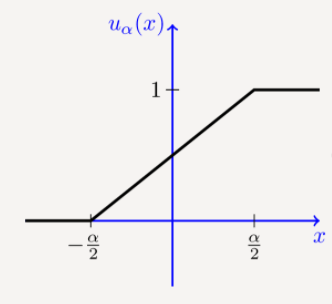
\includegraphics[scale=.7]{step8.PNG}
\label{fig:hsf8}
\end{figure*}

Here is a property to notice, consider reasoning with $lim_{\alpha\rightarrow0} u_{\alpha}(x)$ as you take the limit graphically. Width of the middle piece shrinks but no matter what $\alpha$ value we have, we showed above the linear line must connect to the 0 piece and 1 piece on each end. Thus the slope will have to increase as a result, eventually the elevator doors close so to speak and the linear line will have to slope up to infinity, however that will look like a function we have used before, that is the unit step function itself. Thus we say $lim_{\alpha\rightarrow0} u_{\alpha}(x)=u(x)$. \\

\subsubsection{The New Box $\delta_{\alpha}(x)$}

Now we define a concept with a sub-scripted $\delta_{\alpha}(x)$. Mainly named this due to this being not that far away from the actual Delta function but again these notations go all over the place depending on the textbook, source, professor, classroom, topic, or context that you use it. This is actually just a special case of the box function we had earlier, we define this as step functions and piece wise as

\begin{align*}
    \delta_{\alpha}(x) &= \frac{1}{\alpha}\left[u(t+\frac{\alpha}{2})-u(t-\frac{\alpha}{2})\right]  \qquad \text{or}\\
    \delta_{\alpha}(x) &= \left\{
        \begin{array}{cc}
            \frac{1}{\alpha} &  |x| < \frac{\alpha}{2}  \\
            0 & |x| > \frac{\alpha}{2}.
        \end{array}
    \right.
\end{align*}

Graphically, the box will look like this. 

\pagebreak

\begin{figure*}[!htbp]
\centering
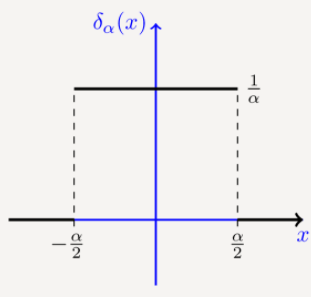
\includegraphics[scale=.7]{step9.PNG}
\label{fig:hsf9}
\end{figure*}

Consider a graphical exercise of integrating this function. If we took $\int_{-\infty}^{\infty} \delta_{\alpha}(x)dx$. Realize all that matters is the middle piece, we have a rectangle, the width is $\frac{\alpha}{2}--\frac{\alpha}{2}=\frac{\alpha}{2}+\frac{\alpha}{2}=\alpha$, the height is $\frac{1}{\alpha}$, that means the area under this curve is 1, thus $\int_{-\infty}^{\infty} \delta_{\alpha}(x)dx=\int_{-\frac{\alpha}{2}}^{\frac{\alpha}{2}} \delta_{\alpha}(x)dx=1$. \\

Here is another good graphical exercise. Consider the derivative of $u_{\alpha}(x)$ in respect to $x$. Reasoning with it graphically we see the connection. Since the slope of the outside segments are 0, and the slope of the linear line is constant, that means we just take the coefficient of $x$ on $\frac{1}{\alpha}\left(x+\frac{\alpha}{2}\right)=\frac{1}{\alpha}x+\frac{1}{2}$ which is $\frac{1}{\alpha}$, that matches the height of our $\delta_{\alpha}(x)$. This means that $\frac{d}{dx}u_{\alpha}(x)=\delta_{\alpha}(x)$.

\begin{figure*}[!htbp]
\centering
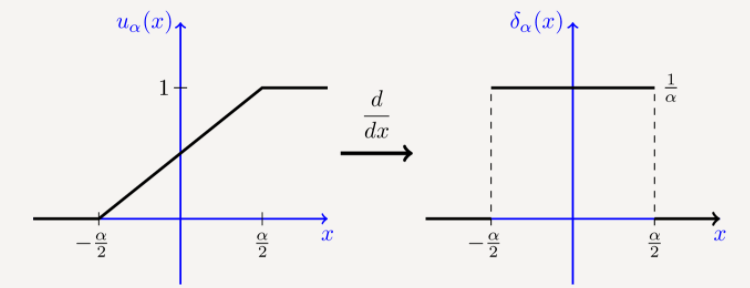
\includegraphics[scale=.7]{step10.PNG}
\label{fig:hsf10}
\end{figure*}

\subsubsection{The Punchline}

Now we are ready to define the Dirac Delta Function and state some facts about it. We will define it as $\delta(x)=lim_{\alpha\rightarrow0} \delta_{\alpha}(x)$. Think about what that will do to the graph. The width of the box shrinks down, however we demonstrated for all values of alpha, that the area of this box must remain 1. So to compensate, the height of the graph must grow as the width of the graph shrinks, continuing down to a width approaching zero because of the limit. This makes something that could vaguely be described piece wise as

\begin{equation*}
    \delta(x)=\left\{
        \begin{array}{cc}
            \infty &  x=0  \\
            0 & \text{otherwise}.
        \end{array}
    \right.
\end{equation*}

This is not the only way to obtain the Dirac Delta Function. We did it by making a unit area box between $\left[-\frac{\alpha}{2},\frac{\alpha}{2} \right]$. Other ways it will happen is some may define it as a box function of $\frac{1}{h}[u(t)-u(t-h)]$, essentially another unit area box but this one only on the positive axis of $[0,h]$, then they define Dirac with taking the limit of $h$ to zero. We briefly mentioned the Normal Distribution in the Gamma Section, those that know stats will sense another way to the Dirac Delta is taking the limit of the Normal's variance going to 0.

\subsection{Fundamental Properties}

\subsubsection{Derivative Connection}

Consider summing up select properties we already found above. We had that the slant like function would limit to the unit step function or $u(x)=lim_{\alpha\rightarrow0} u_{\alpha}(x)$. We had that the derivative of it would be the box function $\frac{d}{dx}u_{\alpha}(x)=\delta_{\alpha}(x)$. Then finally our definition $lim_{\alpha\rightarrow0} \delta_{\alpha}(x)=\delta(x)$. Consider what the derivative of $u(x)$ would be. When we try it, we use the other properties we just stated to see that 

\begin{equation*}
    \frac{d}{dx}u(x)=\frac{d}{dx}lim_{\alpha\rightarrow0} u_{\alpha}(x)=lim_{\alpha\rightarrow0} \frac{d}{dx}u_{\alpha}(x) = lim_{\alpha\rightarrow0} \delta_{\alpha}(x) = \delta(x).
\end{equation*}

There is some hand waving, usually there is a lot of higher level math subtlety when it comes to interchanging a limit and derivative like that, we will just wave our hands and say it works here without spending time trying to justify the swap. This means we now have a major property that $\frac{d}{dx}u(x)=\delta(x)$. We can summarize these concepts now with a pretty nice table.

\begin{center}
  \begin{tabular}{ c  c  c  }
    $u_{\alpha}(x)$  & $\xrightarrow{lim_{\alpha\rightarrow0}}$ & $u(x)$ \\
     $\Bigg\downarrow \frac{d}{dx}$ & & $\Bigg\downarrow \frac{d}{dx}$ \\
     $\delta_{\alpha}(x)$ & $\xrightarrow{lim_{\alpha\rightarrow0}}$ & $\delta(x)$ \\
  \end{tabular}
\end{center}

This is a very nice connection that gets used for deriving so many more properties in applied contexts.

\subsubsection{The Area Conflict}

However we got to the Dirac, notice that since the area of the curve is just a special case of $\delta_{\alpha}(x)$, and we determined that will be an area of 1 for any $\alpha$. That means $\delta(x)$ will also have an area of 1, or otherwise stated in forms like $\int_{-\infty}^{\infty} \delta(x)dx=1$, or $\int_{0-\epsilon}^{0+\epsilon} \delta(x)dx=1$ for any small value of $\epsilon>0$. In the other methods like deriving with the other kind of box function or Normal Distribution, this area of 1 concept also happens there too. \\

If we lead with defining the Dirac Delta without all this wine and dine and just gave the piece wise definition, it would be a tough call to understand how something that only has non zero output at a single $x$ value could have an area other than zero. After all it is a known concept in  Calculus that $\int_{a}^{a}f(t)dt=0$ so why are we allowed to break the rules here? Instead, the piece wise definition loses a lot of subtlety. It is the same light that when we have say a fraction and we take a limit of the denominator going to zero as a different concept as actually dividing by zero, we think of the Dirac Delta Function in the same sense as a limit concept decreasing the width of an interval and not as an explicit one point has a non zero output. Another plausibility to attest why the two facts do not create absurdity is that usually for the same lower and upper limit integral being zero property, our outputs were finite in those regards, however we are now taking an area of a rectangle that has an effective width of zero times an effective height of infinity. From the study of limits, we learned that a limit problem that makes a $0\cdot\infty$ is an indeterminate form, not assumed to be 0. It depended on the problem and how the functions approach 0 and $\infty$ is what determined the limit. \\

With this being a fundamental property, what we do in graphing a Dirac Delta function is different than what we have ever done before. We will not indicate the $y$ value by drawing a vertical line going to infinity at the needed point, but assume we will recall that property and instead draw an arrow segment that stops at the value of the area to remind us how much area the function holds there. 

\pagebreak

\begin{figure*}[!htbp]
\centering
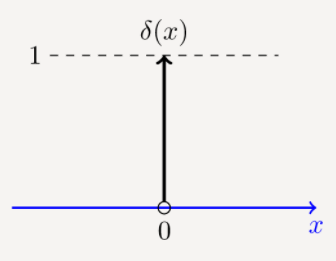
\includegraphics[scale=.8]{step11.PNG}
\label{fig:hsf11}
\end{figure*}

Once we start doing function Transformations momentarily, we will see having this arrow graphical notation will be quite useful. \\

Speaking of functions, as we mentioned in the beginning, the Dirac Delta Function is not technically a function. Without getting into too much detail, a precise deep level definition of a function would lead to different theorems, eventually indicating that a function cannot have these two properties at the same time.

\begin{equation*}
    \delta(x)=0 \quad (\text{for } x\neq0) \qquad \qquad \text{and} \qquad \qquad \int_{-\infty}^{\infty} \delta(x)dx=1.
\end{equation*}

Probably the reason we still call it the Dirac Delta Function is when Nobel Prize winning Physicist Paul Dirac(1902-1984) introduced this concept in his 1930 book The Principles of Quantum Mechanics, he coined at as "Delta Function" back then. 

\subsubsection{Translations}

Here we will see how that arrow graphical technique will really help us. Consider trying to define $\delta(x-x_0)$ for some constant $x_0$. Essentially we are asking to shift the function to the right by $x_0$ units, making the new graph.

\pagebreak

\begin{figure*}[!htbp]
\centering
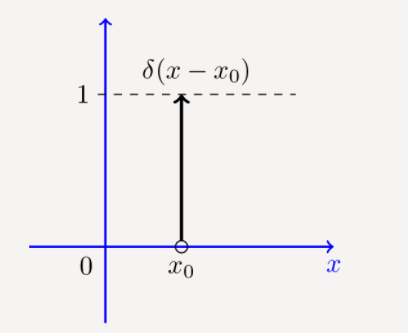
\includegraphics[scale=.8]{step12.PNG}
\label{fig:hsf12}
\end{figure*}

This helps us since we now have our integral specifically at $\int_{-\infty}^{\infty} \delta(x-x_0)dx=\int_{x_0-\epsilon}^{x_0+\epsilon} \delta(x-x_0)dx=1$. \\

Realize what other Transformations would do as well. If we had $f(x)=2\delta(x)$, the integral on this is simply $\int_{-\infty}^{\infty} f(x)dx=\int_{-\infty}^{\infty} 2\delta(x)dx=2\int_{-\infty}^{\infty} \delta(x)dx=2\cdot1=2$, we would graph that by just stretching the arrow up to 2 and labeling said arrow a $2\delta(x-x_0)$. Another nice one addressing the open circle at the beginning of the arrow is graphing say $-1+\delta(x+1)$, here we must start a graph along $y=-1$, then at the point for $x=-1$ we draw an open circle at $(-1,-1)$, then draw an arrow of length 1 straight up to indicate the area. This allows us to freely deal with the Dirac Delta in all its manipulations it will be used for without losing track of its current area. Without it if we just made a bunch of lines going to infinity to indicate the y-value, both a $\delta(x)$ and a $3\delta(x)$ would look the same from our perspective even though their areas are very much different.

\subsubsection{Sifting Property}

Now for one of the best properties of the Dirac Delta, called the Sifting or the Sampling Property, which when used in its applied Math contexts, really makes huge strides. We will show that

\begin{equation*}
    \int_{-\infty}^{\infty} g(x)\delta(x-x_0) dx = g(x_0).
\end{equation*}

First we will define $I=\int_{-\infty}^{\infty} g(x)\delta(x-x_0) dx$, then using $lim_{\alpha\rightarrow0} \delta_{\alpha}(x)=\delta(x)$, we shift it right $x_0$ units to make $lim_{\alpha\rightarrow0} \delta_{\alpha}(x-x_0)=\delta(x-x_0)$ and substitute. We are going to hand wave the swap of limits and integrals, which was the Leibniz Integral Rule, like we did way back in the Laplace of a polynomial section. We will then get

\begin{equation*}
    I=\int_{-\infty}^{\infty} g(x)lim_{\alpha\rightarrow0} \delta_{\alpha}(x-x_0) dx = lim_{\alpha\rightarrow0} \left[\int_{-\infty}^{\infty} g(x) \delta_{\alpha}(x-x_0) dx\right].
\end{equation*}

Now do a quick recall of what $\delta_{\alpha}(x-x_0)$ means, normally $\delta_{\alpha}(x)$ is a box of height $\frac{1}{\alpha}$ for $x$ values between $\left(-\frac{\alpha}{2},\frac{\alpha}{2}\right)$. Now shift that picture $x_0$ units right, to get $\frac{1}{\alpha}$ about $\left(x_0-\frac{\alpha}{2},x_0+\frac{\alpha}{2}\right)$, and everywhere else will output zero. That means we can rewrite this integral by adjusting the limits for the non-zero portion and drop the $\delta_{\alpha}(x-x_0)$ to replace it with its $y$ value for that interval, which is $\frac{1}{\alpha}$. Here we do that to get

\begin{equation*}
    I=lim_{\alpha\rightarrow0} \left[\int_{-\infty}^{\infty} g(x) \delta_{\alpha}(x-x_0) dx\right] = lim_{\alpha\rightarrow0} \left[\int_{x_0-\frac{\alpha}{2}}^{x_0+\frac{\alpha}{2}} \frac{g(x)}{\alpha} dx\right].
\end{equation*}

Time for a little side quest. Recall once upon a  Calculus the Mean Value Theorem. It is when we have a continuous and differentiable function $h(t)$ in an interval from $[a,b]$, then that means there will exist a value $c$ in the interval $[a,b]$ such that $h'(c)=\frac{h(b)-h(a)}{b-a}$. \\

For our problem we state the function, $\int_{x_0-\frac{\alpha}{2}}^{x_0+\frac{\alpha}{2}} \frac{g(x)}{\alpha} dx$, will be continuous and differentiable on the interval $[x_0-\frac{\alpha}{2},x_0+\frac{\alpha}{2}]$. Also we will make an $h(x)=\frac{g(x)}{\alpha}$, with $H(x)$ being the anti-derivative we will luckily not need to find. Notice that means $H\left(x_0-\frac{\alpha}{2}\right)-H\left(x_0+\frac{\alpha}{2}\right)=\int_{x_0-\frac{\alpha}{2}}^{x_0+\frac{\alpha}{2}} \frac{g(x)}{\alpha} dx$. \\

Note the Mean Value Theorem needs a derivative of this integral expression we are using as our function, which being inverses will cancel making $\frac{g(x)}{\alpha}=h(x)$. Then we can claim that there exists a value $x_{\alpha}$ in $[x_0-\frac{\alpha}{2},x_0+\frac{\alpha}{2}]$, that will make

\begin{align*}
     h(x_{\alpha})&=\frac{H(x_0+\frac{\alpha}{2})-H(x_0-\frac{\alpha}{2})}{x_0+\frac{\alpha}{2}-(x_0-\frac{\alpha}{2})} \\
     \frac{g(x_{\alpha})}{\alpha} &= \frac{H(x_0+\frac{\alpha}{2})-H(x_0-\frac{\alpha}{2})}{\alpha} \\
     \frac{g(x_{\alpha})}{\alpha} &= \frac{\int_{x_0-\frac{\alpha}{2}}^{x_0+\frac{\alpha}{2}} \frac{g(x)}{\alpha} dx}{\alpha} \\
     g(x_{\alpha}) &= \int_{x_0-\frac{\alpha}{2}}^{x_0+\frac{\alpha}{2}} \frac{g(x)}{\alpha} dx.
\end{align*}

Back to the $I$ integral, we were at and now we substitute

\begin{equation*}
    I = lim_{\alpha\rightarrow0} \left[\int_{x_0-\frac{\alpha}{2}}^{x_0+\frac{\alpha}{2}} \frac{g(x)}{\alpha} dx\right] = lim_{\alpha\rightarrow0} [g(x_{\alpha})].
\end{equation*}

Now realize as $lim_{\alpha\rightarrow0}$, that narrows the interval that $x_{\alpha}$ is in, the $[x_0-\frac{\alpha}{2},x_0+\frac{\alpha}{2}]$ converges towards the $x_0$ point, this means that $I=lim_{\alpha\rightarrow0} [g(x_{\alpha})]=g(x_0)$. Now since $I=\int_{-\infty}^{\infty} g(x)\delta(x-x_0) dx$ and $I=g(x_0)$ we have finally shown our Sifting Property.

\begin{equation*}
    \int_{-\infty}^{\infty} g(x)\delta(x-x_0) dx = g(x_0).
\end{equation*}

More specifically we could also write this as

\begin{equation*}
    \int_{x_0-\epsilon}^{x_0+\epsilon} g(x)\delta(x-x_0) dx = g(x_0) \qquad \text{for any } \epsilon>0.
\end{equation*}

We can already show some utility this property of Dirac Delta provides. Realize if $g(x)=1$ for all $x$ and the Delta had $x_0=0$, we will see one of our previous results

\begin{equation*}
    \int_{-\infty}^{\infty} [1]\delta(x-0) dx = \int_{-\infty}^{\infty} \delta(x) dx = g(0) = 1.
\end{equation*}

This means this property has special case also providing a second proof that the integral of the Dirac Delta Function is indeed 1. \\

The true utility that this property provides is realize the left side is an integral, a fundamentally continuous concept, the right side is plugging a value at a point, a fundamentally discrete concept. This theorem allows to bridge the gap in a lot of complicated cases nature provides. There are times in nature that we model that are parts continuous and parts discrete. Like for example Quantum Mechanics has electrons that float then once a photon brings energy into the atom the electrons make an instantaneous jump. In Statistics there are concepts that involve distributions that are discrete and continuous at the same time called Mixed distributions and this theorem allows us to write out these concepts with a single equation that we can apply our  Calculus knowledge to rather than a bunch of pieces of a function or cases only described in words.

\subsection{Laplace with Dirac}

We now finally consider the Dirac Delta Function Introduced and perform Laplace study to it.

\subsubsection{Laplace of Dirac}

We will find the Laplace Transform of the Dirac Three different ways. First the harder way, then the amazing way, then an even more amazing way. \\

For the hard way, first we will recall some definitions, the limit definition of Dirac, that $\delta_{\alpha}(x)$ is a box function, and box functions can be written with step functions

\begin{equation*}
    \delta(x)=lim_{\alpha\rightarrow0} \delta_{\alpha}(x)= lim_{\alpha\rightarrow0} \frac{1}{\alpha}\left[u(t+\frac{\alpha}{2})-u(t-\frac{\alpha}{2})\right].
\end{equation*}

Now we take the Laplace Transform, again here we will wave our hands regarding the swap between the implied integral the $\lp$ makes and the limit, it is beyond our abilities

\begin{equation*}
    \lp(\delta(x))= \lp\left(lim_{\alpha\rightarrow0} \frac{1}{\alpha}\left[u(t+\frac{\alpha}{2})-u(t-\frac{\alpha}{2})\right]\right)=lim_{\alpha\rightarrow0} \lp\left(\frac{1}{\alpha}\left[u(t+\frac{\alpha}{2})-u(t-\frac{\alpha}{2})\right]\right).
\end{equation*}

Now we recall our derivation for Laplace of step functions, we have derived that $\lp(c[u(t-a)-u(t-b)])=c\frac{e^{-sa}-e^{-sb}}{s}$ as the very last calculation before the Inverse Laplace of Truncated Functions section. Adapting it for us we have

\begin{equation*}
    \lp(\delta(x))=lim_{\alpha\rightarrow0} \lp\left(\frac{1}{\alpha}\left[u(t+\frac{\alpha}{2})-u(t-\frac{\alpha}{2})\right]\right)=lim_{\alpha\rightarrow0}\frac{1}{\alpha}\frac{e^{s\frac{\alpha}{2}}-e^{-s\frac{\alpha}{2}}}{s}.
\end{equation*}

Now we have a limit problem,

\begin{equation*}
    \lp(\delta(x))=lim_{\alpha\rightarrow0}\frac{e^{\frac{s}{2}\alpha}-e^{-\frac{s}{2}\alpha}}{\alpha s}.
\end{equation*}

Notice we plug $\alpha=0$ to get $\frac{0}{0}$ indeterminate form, then do L'Hopital's rule to get

\begin{equation*}
    lim_{\alpha\rightarrow0}\frac{e^{\frac{s}{2}\alpha}-e^{-s\frac{s}{2}}\alpha}{\alpha s}=lim_{\alpha\rightarrow0}\frac{\frac{s}{2}e^{\frac{s}{2}\alpha}+\frac{s}{2}e^{-\frac{s}{2}\alpha}}{s}.
\end{equation*}

Thankfully this simplifies to $lim_{\alpha\rightarrow0}\frac{1}{2}\left(e^{\frac{s}{2}\alpha}+e^{-\frac{s}{2}\alpha}\right)$, now plug in $\alpha=0$ to get $\frac{1}{2}\left(e^0+e^0\right)=\frac{1}{2}(2)=1$. \\

After all that work we finally say $\lp[\delta(x)]=1$. \\

That may be the proof they take you through in the classroom, however there is an incredibly easier and better way, it all goes back to the Sifting Property. Not only that we will generalize the solve for not just $\delta(x)$, but for $\delta(x-x_0)$ for all positive values of $x_0$, aka any time we shift delta to the right where it affects the Laplace Transform. So by definition

\begin{equation*}
    \lp[\delta(x-x_0)]=\int_{0}^{\infty} \delta(x-x_0) e^{-sx} dx.
\end{equation*}

Recall the theorem is that, 

\begin{equation*}
    \int_{x_0-\epsilon}^{x_0+\epsilon} g(x)\delta(x-x_0) dx = g(x_0) \qquad \text{for any } \epsilon>0.
\end{equation*}

We apply it here where $g(x)=e^{-sx}$, simply plug in the answer for $g(x_0)=e^{-sx_0}$. \\

\begin{equation*}
    \lp[\delta(x-x_0)]= e^{-sx_0}.
\end{equation*}

That is it, that is the proof. Notice when $x_0=0$, that makes $\lp[\delta(x)]=e^{-s(0)}=1$, making a special case of this proving the first derivation we did. \\

Why don't all classrooms show this? Probably comes down to the squeamishness of the proof of the Sifting Property where they do not like hand waving the swap of limits and integrals. If we did put in the effort to prove that swap, this easy proof could very well turn into the hard proof given how involved Leibniz Integral Rule can be. \\

Now for the third way, recall that $\frac{d}{dx}u(x-x_0)=\delta(x-x_0)$, where we assume $x_0>0$ so it shifts to the right meaning the spike is in the Transform's limits. Also recall we had once upon a time a way to relate Laplace Transforms of derivatives with their original functions, that is $\lp[f'(x)]=s\lp[f(x)]-f(0)$. By calling $f(x)=u(x-x_0)$, that means $f'(x)=\delta(x-x_0)$, then we have

\begin{equation*}
    \lp[\delta(x-x_0)]=s\lp[u(x-x_0)]-u(0-x_0).
\end{equation*}

Since $x_0>0$, then $u(x-x_0)=0$ and we are at $\lp[\delta(x-x_0)]=s\lp[u(x-x_0)]$. Now recall we derived $\lp[u(x-x_0)]=\frac{e^{-sx_0}}{s}$, cancelling we see the usual $\lp[\delta(x-x_0)]=s\frac{e^{-sx_0}}{s}=e^{-sx_0}$.

\subsubsection{Dirac and Convolution}

Here we show another clever idea. What if we used the Delta function as an input to the Convolution. That is we wish to calculate

\begin{equation*}
    f(t) \ast \delta(t-a).
\end{equation*}

There are two ways to show this one. Starting with the definition, $f(t) \ast g(t) = \int_{0}^{t} f(u)g(t-u) du$ we have

\begin{equation*}
    \delta(t-a) \ast f(t)= \int_{0}^{t} \delta(t-a)f(t-u) du = \int_{0}^{t} f(t-u)\delta(t-a) du.
\end{equation*}

Note that since $u$ integrate over the limits the values of $u$ satisfy $0\leq u\leq t$, which we will use later. This way we will deal with the Sifting Property, recall it is

\begin{equation*}
    \int_{-\infty}^{\infty} g(t)\delta(t-a) dt = g(a).
\end{equation*}

There are two cases to consider, if $t<a$, then $\delta(t-a)=0$ since $0\leq u\leq t<a$, otherwise said that the spike happens to the right of the value $t$ in our $0$ to $t$ integral making it zero, abbreviated as $\int_{0}^{t} f(t-u)\delta(t-a) du=0$. \\

The remaining case is $t\geq a$, or that the spike is in range of the Convolution integral, that means since the spike is in range of both the Sifting property and the Convolution, we change the limits so they both agree by being around the spike at $a$. Then to match our integrands up, we say that $g(t)$ in the Sifting will substitute to match $g(t)=f(t-u)$ for us, that means when we do $u=a$ and makes

\begin{equation*}
     \int_{0}^{t} f(t-u)\delta(t-a) du = f(t-a).
\end{equation*}

So with both cases in mind that writes out as a piece wise function of

\begin{equation*}
    f(t) \ast \delta(t-a) = \left\{
        \begin{array}{cc}
            0 &  t<a  \\
            f(t-a) &  t\geq a.
        \end{array}
    \right.
\end{equation*}

However this is also known as with the step function, $u(t-a)f(t-a)$. We can write this succinctly as $f(t) \ast \delta(t-a)=u(t-a)f(t-a)$. \\

The second and probably better way to do it is to think in terms of Convolutions for Laplace Transforms. Consider taking the Laplace Transform of $f(t) \ast \delta(t-a)$. Since we learned Convolution is just the product of the individual Transforms, that makes $\lp[f(t)]=F(s)$ and also we bring back a previously proven property of $\lp[\delta(t-a)]=e^{-as}$. This means

\begin{equation*}
    \lp[f(t) \ast \delta(t-a)] = F(s)\cdot e^{-as}. 
\end{equation*}

However, also recall another previously proven step function Laplace property

\begin{equation*}
    \lp[u(t-a)f(t-a)]=e^{-sa}\lp[f(t)].
\end{equation*}

So both $f(t) \ast \delta(t-a)$ and $u(t-a)f(t-a)$ have the same Laplace Transform, therefore by the Uniqueness Theorem of Laplace, we have that $f(t) \ast \delta(t-a) = u(t-a)f(t-a)$ yet again.

\subsubsection{Dirac and Step Functions in Differential Equations}

Here we will show an example of Dirac and a Step function involved in a differential equation. Consider trying to solve

\begin{equation*}
    y"+2y'-15y=6\delta(t-9), \qquad \qquad y(0)=-5 \quad y'(0)=7
\end{equation*}

When would we see a Differential Equation like this in the real world? It can definitely happen, an example of a second order system can be like a pendulum problem or a spring system, maybe the physics involved Hook's Law. Anyway the right hand side is also a consideration of an outside force being put on the system. So what would have a Dirac Delta function? There is a physics concept for an example called an Impulse, an Impulse is defined as an integral of Force over Time, different from Work which integrates Force over Distance. A Unit Impulse or a Force that happens in a blink of an eye like a collision would be modeled with a Dirac Delta Function. Here we see 9 units of time into this equation starting its physical system, we will essentially slap 6 units of force instantaneously into the system, maybe someone threw a rock at a moving spring or something. \\

We do not see the unit step function but it will come in the solution later. Consider taking the Laplace Transform of both sides.

\begin{align*}
    \lp[y"+2y'-15y] &= \lp[6\delta(t-9)] \\
    \lp[y"]+2\lp[y']-15\lp[y] &= 6\lp[\delta(t-9)] \\
    s^2\hugey -sy(0)-y'(0)+2(s\hugey-y(0))-15\hugey &= 6e^{-9s} \\
    (s^2+2s-15)\hugey+5s+3 &= 6e^{-9s} \\
    \hugey = \frac{6e^{-9s}}{(s+5)(s-3)}&-\frac{5s+3}{(s+5)(s-3)}.
\end{align*}

For sake of communication, we will call this $\hugey = 6e^{-9s}F(s)-G(s)$, with $F(s)=\frac{1}{(s+5)(s-3)}$ and $G(s)=\frac{5s+3}{(s+5)(s-3)}$. In anticipation of setting up the Laplace Inverse, we will do partial fractions here. First we start with partial fractions of $F(s)$ and take the inverse Laplace of it to get an $f(t)$,

\begin{equation*}
    F(s)=\frac{1}{(s+5)(s-3)} = \frac{\frac{1}{8}}{s-3}-\frac{\frac{1}{8}}{s+5}.
\end{equation*}

The inverse being $\lp^{-1}[F(s)]=f(t)$ will make

\begin{equation*}
    f(t)=\frac{1}{8}\lp^{-1}\left[\frac{1}{s-3}\right]-\frac{1}{8}\lp^{-1}\left[\frac{1}{s+5}\right]=\frac{1}{8}e^{3t}-\frac{1}{8}e^{-5t}.
\end{equation*}

That part complete we will partial fraction and inverse $G(s)$ now.

\begin{equation*}
    G(s)=\frac{5s+3}{(s+5)(s-3)}=\frac{\frac{9}{4}}{s-3}+\frac{\frac{11}{5}}{s+5}.
\end{equation*}

Now take the inverse $\lp[G(s)]=g(t)$ to get

\begin{equation*}
    g(t)=\frac{9}{4}\lp^{-1}\left[\frac{1}{s-3}\right]+\frac{11}{5}\lp^{-1}\left[\frac{1}{s+5}\right]=\frac{9}{4}e^{3t}+\frac{11}{5}e^{-5t}.
\end{equation*}

Now that we have found the inverse of some parts, let's try the inverse of the whole, notice we have the unit step function entry of $\lp[u(t-c)f(t-c)]=e^{-sc}\lp[f(t)]$ is in play for the inverse of $e^{-9s}F(s)$, this will make

\begin{align*}
    \hugey &= 6e^{-9s}F(s)-G(s) \\
    y(t) &= 6u(t-9)f(t-9)-g(t).
\end{align*}

With this being $f(t)$ and $g(t)$ being defined above. That makes 

\begin{equation*}
    y(t) = 6u(t-9)\left[\frac{1}{8}e^{3(t-9)}-\frac{1}{8}e^{-5(t-9)}\right]-\left[\frac{9}{4}e^{3t}+\frac{11}{5}e^{-5t}\right]
\end{equation*}

Realize what this solution looks like, we have a system that was chugging along from $t=0$ to $t=9$, suddenly an outside force, a impulse of 6 impacts the system and it suddenly changes how it moves, that is sensible since we have a unit step function at $t=9$ in our solution activates the other term so it turns the function describing the movement of our solution into a completely different function. This is a big connection between the Dirac Delta and the Unit Step function when thinking in terms of nature and Physics. It makes sense if you punch a moving target, its movement will suddenly change.

\section{Conclusion and Tables}

There is still plenty more to Laplace Transforms, this usually covers most or probably all and then some of what would be seen in lecture portions to an intro Differential Equations class. They can also be used to solve systems of Differential Equations, without doing an example it simply put turns multiple Differential Equations into multiple algebraic equations. Then you solve that algebraic system of equations and inverse Laplace those back to get the solution. \\

Later they sometimes get employed to solve Partial Differential Equations. The technique of Laplace Transforms gets generalized later too. In a Partial Differential Equations class you see the concept of a Fourier Transform which is another level of power in a Transform, it involves some imaginary number work in its integrand so it is a level of complexity beyond the Laplace but it is much more powerful. \\

With that said here is the final minimalist entry table for what we have covered here, if you do not feel comfortable with combining entries to solve your problem, we suggest to make your own table with extra entries. Again, these table are personal preference between a trade off of how big the table gets making it harder to search through vs. how much mental effort it takes to combine multiple entries to solve a problem. \\

Also we made a table for properties and definitions of the Applied functions we discussed that do not have Laplace explicitly mentioned in the equation. Though some were proven using Laplace Techniques.



\begin{center}
\small
    \begin{tabular}{|l|c|}
    \hline
    1. \qquad 1 & $\frac{1}{s}$ \\
    \hline \hline
    2. \qquad $f(t)+g(t)$ & $F(s)+G(s)$  \\
    \hline \hline
    3. \qquad $cf(t)$ & $cF(s)$ \\
    \hline \hline
    4. \qquad $e^{at}f(t)$ & $F(s-a)$  \\
    \hline \hline
    5. \qquad $cos(at)$ & $\frac{s}{(s^2+a^2)}$ \\
    \hline \hline
    6. \qquad $sin(at)$ & $\frac{a}{(s^2+a^2)}$ \\
    \hline \hline
    7. \qquad $t^n$ & $\frac{n!}{s^{n+1}}$ \\
    \hline \hline
    8. \qquad $t^n \cdot f(t)$ & $(-1)^n\frac{d^n}{ds^n}F(s)$ \\
    \hline \hline
    9. \qquad $f'(t)$ & $sF(s)-f(0)$ \\
    \hline \hline
    10. \qquad $f''(t)$ & $s^2F(s)-sf(0)-f'(0)$ \\
    \hline \hline 
    11. \qquad $f^{(n)}(t)$ & $s^nF(s)-s^{n-1}f(0)-s^{n-2}f'(0) \ldots -sf^{(n-2)}(0)-f^{(n-1)}(0)$ \\
    \hline \hline
    12. \qquad $f(t)=f(t+T)$ & $\frac{\int_{0}^{T} f(t) e^{-st} dt}{1-e^{-sT}}$ \\
    \hline \hline
    13. \qquad $t^{\alpha}$ for real number $\alpha$ & $\frac{\Gamma(\alpha+1)}{s^{\alpha+1}}$ \\
    \hline \hline
    14. \qquad $f(t) \ast g(t) = \int_{0}^{t} f(u)g(t-u) du$ & $F(s)\cdot G(s)$ \\
    \hline \hline
    15. \qquad $u(t-c)f(t-c)$ & $e^{-sc}\lp[f(t)]$ \\
    \hline \hline
    16. \qquad $\delta(x-c)$ & $e^{-sc}$ \\
    \hline
\end{tabular}
\end{center}


\pagebreak

\begin{table}
\small
    \begin{tabular}{|l|l|}
    \hline
    1. Exist $T$ such that for all $t$, $f(t)=f(t+T)$. & (Periodic Definition) \\
    \hline \hline
    2. $1+x+x^2+x^3+\ldots+x^n=\frac{1-x^{n+1}}{1-x}$ & (Finite Geometric Series) \\
    \hline \hline
    3. $1+x+x^2+x^3+\ldots= \frac{1}{1-x} \qquad \text{when} \qquad |x|<1$ & (Infinite Geometric Series) \\
    \hline \hline
    4. $\Gamma(\alpha)=\int_{0}^{\infty}y^{\alpha-1}e^{-y}dy$ & (Gamma Function Definition) \\
    \hline \hline
    5. $\Gamma(\alpha) = (\alpha -1) \Gamma(\alpha -1)$ & (First Gamma Prop.)  \\
    \hline \hline
    6. $\Gamma(1)=1$ & (Second Gamma Prop.) \\
    \hline \hline
    7. $\Gamma(n) = (n-1)!$ & (Third Gamma Prop.)  \\
    \hline \hline
    8. $\Gamma\left(\frac{1}{2}\right)=\sqrt{\pi}$ & (Fourth Gamma Prop.) \\
    \hline \hline
    9. $\int_{-\infty}^{\infty} e^{\frac{-x^2}{2}} dx=\sqrt{2\pi}$ & (Gaussian Integral)  \\
    \hline \hline
    10. $(x+y)^n = \sum_{r=0}^{n} \binom{n}{r} x^{n-r}y^r$  & (Binomial Theorem) \\
    \hline \hline
    11. $\left(\sum_{n=0}^{\infty} a_n x^n\right)\cdot \left(\sum_{n=0}^{\infty} a_n x^n\right)=\sum_{n=0}^{\infty} \left[\sum_{k=0}^n a_{k}b_{n-k}\right] x^n$ & (Power Series Convolution) \\
    \hline
    \end{tabular}
\end{table}
    
\begin{table}
\small
    \begin{tabular}{|l|l|}
    \hline
    12. $f(t) \ast g(t) = \int_{0}^{t} f(u)g(t-u) du$ & (Definition Continuous Convolution)  \\
    \hline \hline
    13. $f(t) \ast 1 = \int_{0}^{\infty} f(u)du$ & (1 is not Convolution Identity)  \\
    \hline \hline
    14. $f(t) \ast 0 = 0$ & (Zero Convolution)  \\
    \hline \hline
    15. $a[f(t) \ast g(t)] = [af(t)] \ast g(t)$ & (Associative with Scalar Mult.)  \\
    \hline \hline
    16. $f(t) \ast g(t) = g(t) \ast f(t) $ & (Convolution Commutative)  \\
    \hline \hline
    17. $(f(t) \ast g(t)) \ast h(t) = f(t) \ast (g(t) \ast h(t))$ & (Convolution Associative)  \\
    \hline \hline
    18. $f(t) \ast (g_1(t)+g_2(t)) = f(t) \ast g_1(t) + f(t) \ast g_2(t)$ & (Convolution Distributive)  \\
    \hline \hline
    19. $\beta(a,b) = \int_{0}^{1} (1-x)^{a-1}(x)^{b-1} dx$ & (Definition Beta Function)  \\
    \hline \hline
    20. $\beta(a,b) = \frac{\Gamma(a)\Gamma(b)}{\Gamma(a+b)}$ & (Beta Gamma Connection) \\
    \hline \hline
    21. $u(x)=\left\{
        \begin{array}{rl}
            1 &  x \geq 0  \\
            0 &  x < 0.
        \end{array}
    \right.$ & (Definition Step Function) \\
    \hline \hline
    22. $u(t-c)$ & (Left Right Shift Step) \\
    \hline \hline
    23. $cu(t)$ & (Vertical Stretch Step) \\
    \hline \hline
    24. $u(t-c)f(t)$ & (Off-On switch $f(t)$ at $c$.) \\
    \hline \hline
    25. $c[u(t-a)-u(t-b)]$ & (Box between $[a,b]$ height c) \\
    \hline \hline
    26. $u_{\alpha}(x)=\left\{
        \begin{array}{cc}
            0 &  x < -\frac{\alpha}{2}  \\
            \frac{1}{\alpha}\left(x+\frac{\alpha}{2}\right) &  -\frac{\alpha}{2} \leq x \leq \frac{\alpha}{2} \\
            1 & x > \frac{\alpha}{2}.
        \end{array}
    \right.$ & (Slant function def) \\
    \hline \hline
    27. $\delta_{\alpha}(x) = \frac{1}{\alpha}\left[u(t+\frac{\alpha}{2})-u(t-\frac{\alpha}{2})\right]$ & (Box Delta) \\
    \hline \hline
    28. $\delta(x)=lim_{\alpha\rightarrow0} \delta_{\alpha}(x)$ & (Definition Dirac Delta) \\
    \hline \hline
    29. $\delta(x)=\left\{
        \begin{array}{cc}
            \infty &  x=0  \\
            0 & \text{otherwise}.
        \end{array}
    \right.$ & (Alt. Definition) \\
    \hline \hline
    30. $lim_{\alpha\rightarrow0}=u_{\alpha}(x)=u(x)$ & (Slant Limits to Unit Step) \\
    \hline \hline
    31. $\frac{d}{dx}u_{\alpha}(x)=\delta_{\alpha}(x)$ & (Slant Derivative is Delta Box) \\
    \hline \hline
    32. $\frac{d}{dx}u(x)=\delta(x)$ & (Unit Step Derivative is Dirac) \\
    \hline \hline
    33. $\int_{-\infty}^{\infty} \delta_{\alpha}(x)dx=\int_{-\frac{\alpha}{2}}^{\frac{\alpha}{2}} \delta(x)dx=1$ & (Delta Box Area 1)  \\
    \hline \hline
    34. $\int_{-\infty}^{\infty} \delta(x)dx=\int_{0-\epsilon}^{0+\epsilon} \delta(x)dx=1$ & (Dirac Area 1) \\
    \hline \hline
    35. $\delta(x-a)$ & (Delta left right shift) \\
    \hline \hline
    36. $c\delta(x)$ & (Delta area scales by c) \\
    \hline \hline
    37. $\int_{-\infty}^{\infty} g(x)\delta(x-x_0) dx = g(x_0)$ & (Sifting Property) \\
    \hline \hline
    38. $f(t) \ast \delta(t-a) = u(t-a)f(t-a)$ & (Dirac in Convolution) \\
    \hline \hline
    39. $f(t) \ast \delta(t) = f(t)$ (Special case 31) & (Dirac Identity element of Convolution) \\
    \hline
\end{tabular}
\end{table}



\end{document}
